% Emit warnings on deprecated things.
\RequirePackage[l2tabu, orthodox]{nag}

\documentclass{scrreprt}

% Load custom packages+settings and commands.
\usepackage{style_and_commands/style}
% Project related.
  % Project information.
  \newcommand{\projecttitle}{Some name}
  \newcommand{\projecttheme}{Developing Complex Software Systems}
  \newcommand{\projectperiod}{Spring semester 2015}
  \newcommand{\projectcopies}{8}
  \newcommand{\projectcompletion}{May 27, 2015}

  % Names.
  \newcommand{\groupname}{sw609f15}
  \newcommand{\supervisor}{Kim A. Jakobsen} % no \@ here!
  \newcommand{\groupmembersbyfirstname}[0]{%
    Andreas Petersen\\
    Mads Ellersgaard Kalør\\
    Michael Toft Jensen\\
    Søren Bøtker Ranneries
  }

% Custom styling commands.
  % Monospaced text.
  \newcommand*\justify{%
    \fontdimen2\font=0.4em% interword space
    \fontdimen3\font=0.2em% interword stretch
    \fontdimen4\font=0.1em% interword shrink
    \fontdimen7\font=0.1em% extra space
    \hyphenchar\font=`\-% allowing hyphenation
  }
  \newcommand{\mono}[1]{\texttt{\justify #1}}

  % Chapter introductions.
  \newcommand{\chapterintro}[1]{#1}
  
  % Group X.
  \newcommand{\group}[1]{Group #1}
  
  % User story.
  \newcommand{\us}[1]{\emph{#1}}
  
  % Project names
  \newcommand{\gproject}[1]{#1}
  
  % Subproject names
  \newcommand{\gui}{GUI\@\xspace} \newcommand{\guititle}{GUI\xspace}
  \newcommand{\db}{DB\@\xspace} \newcommand{\dbtitle}{DB\xspace}
  \newcommand{\bd}{B\&D\@\xspace} \newcommand{\bdtitle}{B\&D\xspace}

  % CD paths with icon.
  \newcommand{\cdpath}[1]{%
    % Param1: path
    \hyperref[app:cd]{\raisebox{-0.28ex}{
\includegraphics[height=0.85em]{cd}}\mono{/#1}}%
  }

  % Margin text.
  \newcommand{\margintext}[1]{\marginline{\textsf{\footnotesize #1}}}
  
  \newcommand{\code}[1]{#1}
  
  % Todo.
  \newcommand{\todo}[1]{\fxnote{#1}}
  \FXRegisterAuthor{kim}{notsameaskim}{\color{blue}Kim}
  
  % Dummy line.
  \newcommand{\dummy}{\todo{Lorem ipsum dolor sit amet, consectetur adipiscing elit.}}

% Document structure.
  % Sprints.
  \newcounter{sprintcounter}%\addtocounter{sprintcounter}{1}
  \newcommand{\sprint}[1]{%
    \stepcounter{sprintcounter}
    \part*{Sprint \arabic{sprintcounter}\\\vspace{1cm}\textnormal{\textsf{#1}}}
    \addcontentsline{toc}{part}{Sprint \arabic{sprintcounter}: #1}
  }
  
  % Chapter grouping.
  \newcommand{\chaptergroup}[1]{
    \part*{#1}
    \addcontentsline{toc}{part}{#1}
  }
  
  % Document organization.
  \newenvironment{documentorganization}
    {\vspace{.5cm}\noindent\textbf{Report Organization}\quad The remainder of this report is organized in the following fashion:\begin{itemize}}
    {\end{itemize}}
  
  % Chapter organization.
  \newenvironment{chapterorganization}
    {\vspace{.5cm}\noindent\textbf{Chapter Organization}\quad The remainder of this chapter is organized in the following fashion:\begin{itemize}}
    {\end{itemize}}
    
   % Abbreviation.
  \newenvironment{abbreviations}
    {\vspace{.5cm}\noindent\textbf{Chapter Abbreviations}\quad This chapter introduces the following abbreviations:\begin{addmargin}[\leftmargin]{0em}\begin{multicols}{2}\begin{description}[noitemsep, style=sameline]}
    {\end{description}\end{multicols}\end{addmargin}}
    
    % Dates.
    \newenvironment{dates}
    {\vspace{.5cm}\noindent\textbf{Project Dates}\quad \dummy:\begin{addmargin}[\leftmargin]{0em}\begin{multicols}{2}\begin{description}[noitemsep, style=sameline]}
    {\end{description}\end{multicols}\end{addmargin}}

% Figures.
  % Normal figure.
  \newcommand{\fig}[3]{
    \begin{figure}[tbp]
      \centering
      %\rule{\textwidth}{0.005in}
      \includegraphics[width=0.75\textwidth]{#1}
      \caption[#2]{#3}\label{fig:#1}
      %\rule{\textwidth}{0.005in}
    \end{figure}
  }
  
  % Scaled figure.
  \newcommand{\figscaled}[4]{
    \begin{figure}[tbp]
      \centering
      \includegraphics[scale=#4]{#1}
      \caption[#2]{#3}\label{fig:#1}
    \end{figure}
  }
  
  % Figure with custom width.
  \newcommand{\figcustomwidth}[4]{
    \begin{figure}[tbp]
      \centering
      \includegraphics[width=#4]{#1}
      \caption[#2]{#3}\label{fig:#1}
    \end{figure}
  }

% References.
  \newcommand{\appendixref}[1]{\hyperref[#1]{Appendix \ref*{#1}}}
  \newcommand{\chapterref}[1]{\hyperref[#1]{Chapter \ref*{#1}}}
  \newcommand{\sectionref}[1]{\hyperref[#1]{Section \ref*{#1}}}
  \newcommand{\figureref}[1]{\hyperref[#1]{Figure \ref*{#1}}}
  \newcommand{\tableref}[1]{\hyperref[#1]{Table \ref*{#1}}}
  \newcommand{\listingref}[1]{\hyperref[#1]{Listing \ref*{#1}}}
  \newcommand{\onpage}[1]{on \hyperref[#1]{page \pageref*{#1}}}
  \newcommand{\equationref}[1]{\hyperref[#1]{Equation \ref*{#1}}}
  \newcommand{\algorithmref}[1]{\hyperref[#1]{Algorithm \ref*{#1}}}
  %\newcommand{\sprintref}[1]{\hyperref[#1]{Sprint \ref*{#1}}}

% Column types for tabulars.
%\newcolumntype{L}[1]{>{\raggedright\let\newline\\\arraybackslash\hspace{0pt}}m{#1}}
%\newcolumntype{R}[1]{>{\raggedleft\let\newline\\\arraybackslash\hspace{0pt}}m{#1}}

% Fix todo notes with externalize
\let\oldTodo\todo
\renewcommand{\todo}[1]{\tikzexternaldisable{}\oldTodo{#1}\tikzexternalenable{}}

% Fixme stuff.
%\newcommand{\fillin}[1]{\fxnote*[inline]{#1}{Fill in: }}

% Vector command.
%\newcommand{\omatrix}[1]{\ensuremath{\boldsymbol{#1}}}

% A better plus minus sign.
\makeatletter
\newcommand{\gpm}{\mathbin{\mathpalette\@gpm\relax}}
\newcommand{\@gpm}[2]{\ooalign{%
  \raisebox{.1\height}{$#1+$}\cr
  \smash{\raisebox{-.6\height}{$#1-$}}\cr}}
\makeatother


% Set custom settings
  % Set true for PDF version ready for print. False for screen version.
  \settoggle{printversion}{false}

\begin{document}

%\linenumbers

% Cover page.
\let\oldthepage\thepage{}
\renewcommand\thepage{Cover}
\bookmark[page=1,level=0]{Cover}
\tikzexternaldisable{}

\includepdf[pages=-]{frontmatter/frontpage.pdf}
\tikzexternalenable{}
\renewcommand\thepage{\oldthepage}

\hypersetup{pageanchor=false} % To avoid problems with hyperref package
\thispagestyle{empty}
{\small
\strut\vfill
\noindent \copyright{} \groupname{}, Aalborg University, \MakeLowercase{\projectperiod{}}.\par
\vspace{0.3cm}
%\noindent Here you can write something about which tools and software you have used for typesetting the document, running simulations and creating figures. If you do not know what to write, either leave this page blank or have a look at the colophon in some of your books.\par
%\vspace{0.2cm}
}
\clearpage
\hypersetup{pageanchor=true} % Reenable this.

% Start roman numbering.
\cleardoublepage{}
\pagenumbering{roman}
\setcounter{page}{1}

\bookmark[page=3,level=0]{Title Page}
{
    %set up various length
    \ifx\titlepageleftcolumnwidth\undefined{}
      \newlength{\titlepageleftcolumnwidth}
      \newlength{\titlepagerightcolumnwidth}
    \fi
    \setlength{\titlepageleftcolumnwidth}{0.42\textwidth-\tabcolsep}
    \setlength{\titlepagerightcolumnwidth}{\textwidth-2\tabcolsep-\titlepageleftcolumnwidth}
    %create title page
    \thispagestyle{empty}
    \noindent%
    \begin{tabular}{@{}ll@{}}
      \parbox{0.97\titlepageleftcolumnwidth}{
          
\includegraphics[width=0.97\titlepageleftcolumnwidth]{aau_logo_en}
      } &
      \vspace{1cm}
      \parbox{0.97\titlepagerightcolumnwidth}{\raggedleft\sffamily\small
        \textbf{\color{sectioning}Department of Computer Science}\\
        Selma Lagerlöfs Vej 300\\
        DK-9220 Aalborg Ø\\
        \href{http://www.cs.aau.dk}{http://www.cs.aau.dk}
      }\bigskip\\
        \parbox[t]{\titlepageleftcolumnwidth}{
        \textbf{\color{sectioning}\sffamily{Title:}}\\ \projecttitle{}\bigskip\par
        \textbf{\color{sectioning}\sffamily{Theme:}}\\ \projecttheme{}\bigskip\par
        \textbf{\color{sectioning}\sffamily{Project period:}}\\ \projectperiod\bigskip\par
        \textbf{\color{sectioning}\sffamily{Project group:}}\\ \groupname{}\bigskip\par
        \textbf{\color{sectioning}\sffamily{Participants:}}\\ \groupmembersbyfirstname{}\bigskip\par
        \textbf{\color{sectioning}\sffamily{Supervisor:}}\\ \supervisor\bigskip\par
        \textbf{\color{sectioning}\sffamily{Copies:}} \projectcopies\bigskip\par
        \textbf{\color{sectioning}\sffamily{Pages:}}~\pageref*{LastPageLabel}\bigskip\par
        \textbf{\color{sectioning}\sffamily{Date of completion:}}\\ \projectcompletion
  } &
      \parbox[t]{0.97\titlepagerightcolumnwidth}{%
      \textbf{\color{sectioning}\sffamily{Abstract:}}\smallskip\par{}
        \fbox{\parbox{0.97\titlepagerightcolumnwidth-2\fboxsep-2\fboxrule}{%
          Continuous integration in a complex software suite is challenging. We present a configuration of continuous integration and development method for a large team of \nth{6} semester Software Engineering students at Aalborg University working on the GIRAF Android apps aimed at easing the lives of people with Autism Spectrum Disorders and their caretakers. The project is organized according to Scrum of Scrums, comprising 15 groups of 1--4 persons. The code base is inherited from previous semesters. We setup a tool, Jenkins, to automatically build and test apps and libraries that are developed by the project, whenever changes are made. The apps are automatically tested on physical tablets wirelessly and uploaded to Google Play. Libraries are automatically published to a Maven repository saving all built versions. We run automated monkey tests on all GIRAF apps, filling the database with dummy data with an app before starting and blocking the Android notification bar to avoid changing settings. We have significantly improved the build environment compared to what we started with.
        }}
      }\\
    \end{tabular}
    \vfill
      \noindent{\footnotesize\emph{The content of this report is freely available, but publication (with reference) may only be pursued due to agreement with the authors.}}
    \clearpage
  }

\thispagestyle{empty}
\vspace*{\fill}
\noindent
\sffamily
%
\rule{9cm}{1pt}\\
\vspace{1.5cm}
Andreas Petersen\\
%
\rule{9cm}{1pt}\\
\vspace{1.5cm}
Mads Ellersgaard Kalør\\
%
\rule{9cm}{1pt}\\
\vspace{1.5cm}
Michael Toft Jensen\\
%
\rule{9cm}{1pt}\\
\vspace{1.5cm}
Søren Bøtker Ranneries\\
%
\normalfont
\vspace*{\fill}
\bookmark[page=5,level=0]{Preface}
\chapter*{Preface}
This report is a product of a bachelor project by four Software students at Aalborg University. The title of this semester project is \projecttheme.

It is expected that the reader has a knowledge of computer science at the same level as a 6\textsuperscript{th} semester Software student at Aalborg University in order for the reader to benefit the most from reading this report.\par
\begingroup % Next chapter on same page.
\let\cleardoublepage\relax
\bookmark[page=5,level=0]{Reading Guide}
%!TEX root = ../report.tex
\chapter*{Reading Guide}
The report is comprised of several parts. There is a preliminary part which describes the framework for the project. There are four sprint parts, which chronologically details the work done during the project. The last part contains an evaluation, conclusion, and recommendations for future developers. Developers of next year will mostly be interested in the first and the last part.

Personal pronouns refer to the authors of this report. All figures in the report are made by the authors.

\section*{Citation Style}
All references throughout the report are in IEEE style. Every source in lexicographical order is assigned the consecutive number in which it is referred to. The bibliography can be found at the end of this report \onpage{bibliography}.

%\section*{Disc}
%A disc is supplied in [insert disc ref]. Explain more... %The use of ``\cdpath{}'' refers to the root of the disc. The disc contains source code for all parts of the project as well as this report in PDF format.

%\section*{Source Code}
\endgroup

% Table of contents.
\bookmark[page=7,level=0]{Contents}
\microtypesetup{protrusion=false} % Protrusion may interfere with the dotted lines in the TOC.
\ohead{{\MakeUppercase\leftmark}} % UGLY HACK. The correct way should be to store the old value, set new value, then restore old value!
\tableofcontents
\microtypesetup{protrusion=true}

% Start arabic numbering and restore page header.
\cleardoublepage{}
\ohead{{\MakeUppercase\leftmark}\rightmark}
\pagenumbering{arabic}

% Main content.
\chaptergroup{Preliminaries}
\chapter{Introduction}
\kimnote{Et projekt skal starte med en general forklaring af problemstillingen i den virklige verden. Derefter kan i nævne formelle ting.}
The purpose of this semester project is to develop a complex software system in a large development environment. The software system is called GIRAF (Graphical Interface Resources for Autistic Folk) and is inherited from the 6\textsuperscript{th} semester students of past years. The project is a collaboration between Aalborg University, Aalborg Municipality and several institutions that work with autistic citizens. 
\kimnote{I skal beskrive hvem der præcis er jeres kunder og ikke bare nogle af dem. Det er nok bedst er flytte sådan en redegørelse et andet sted hen.}

The GIRAF project was initiated by Ulrik Nyman, Associate Professor at Aalborg University, in 2011. It is a software suite aimed at easing the daily routines of autistic citizens and their guardians. Autistic citizens generally have limited language skills and thus their primary way of communicating is through pictograms. An important aspect of the multi-project is therefore easing this communication.

Most are Android apps.
The project consists of several front-end and back-end subprojects, that each serves a purpose of the combined system. Most of the Examples of the subprojects are \todo{Insert example applications with brief description}.

\begin{description}
  \item[Launcher] \dummy
  \item[Sekvens]
  \item[Pictooplæser]
	\item[Kategoriværktøjet] \dummy
  \item[Picto Creator] Hvad er dette?
  \item[Pictotegner]
  \item[Picto Search] \dummy
  \item[Oasis App]
  \item[Ugeplan]
  \item[Tidstager] 
  \item[Stemmespillet]
  \item[Kategorispillet]
  \item[Web Ugeplan]
  \item[Webadmin]
\end{description}
\todo{This list are the front-end apps. Maybe move to appendix?}
\kimnote{Forklar det der er essentielt for jeres projekt. Det kunne være fint med en liste over de andre "projekter" i appendix, men brug kun tid på det hvis det bringer værdi til jeres projekt. Det der skal stå i en rapport er hvad i har lavet krydret en passende mængde context.}

There are 14 project groups with approximately 4 students in each. It is crucial that project groups work towards creating a working system, and to allow this a common work process has been decided by the semester coordinator. As such, the semester is split into four sprints (in Scrum terms). \kimnote{I bør introducere jeres process(scrum) før i begynder at bruge fagtermer fra den. Det er nok med et par linjer her i intruduktionen hvor i skriver at i bruger scrum. Jeg tror det vil gavne jer at have en kort sektion om jeres adoptering af scrum, altså hvilke scrum værktøjer i bruger, medmindre i bruger ren scrum!}
The organization of this report reflects these sprints. \todo{Write more about early process decisions.}

\begin{documentorganization}
  \item In \chapterref{chap:sw_dev_method} we describe the software development method used across the multi-project as well as in our group;
  \item Sprint 0:
  \begin{itemize}
    
    \item In \chapterref{chap:sprint1_planning} we describe the sprint planning process;
    \item In \chapterref{chap:config_management} we describe our responsibility as the configuration management group;
    \item In \chapterref{chap:sprint1_end} we describe and conclude on the sprint. 
  \end{itemize}
  \item Sprint 1:
  \begin{itemize}
    \item \todo{Fill Sprint 1 content in.}
  \end{itemize}
  \item Sprint 2:
  \begin{itemize}
    \item \todo{Fill Sprint 2 content in.}
  \end{itemize}
  \item Sprint 3:
  \begin{itemize}
    \item \todo{Fill Sprint 3 content in.}
  \end{itemize}
\end{documentorganization}

\todo{Skriv noget om ``external customer'' da vi også har ``internal customers''}
%!TEX root = ../report.tex
\chapter{Software Development Method}\label{chap:sw_dev_method}
One of the great challenges this semester is to coordinate the development process across all 15 groups. This chapter defines the development method as it looks at the end of the project.

\begin{chapterorganization}
  \item in \sectionref{sec:project_overview} we describe how the multi-project is organized and introduce the hierarchy of the project;
  \item in \sectionref{sec:swmethod_ourgroup} we describe the software development method in our group;
  \item in \sectionref{sec:multi_project_group_roles} we detail the responsibilities delegated to specific groups.
\end{chapterorganization}

\begin{abbreviations}
  \item[\gui] Graphical User Interface
  \item[\db] Database
  \item[\bd] Build \& Deployment
  \item[PO] Product Owner
\end{abbreviations}

\section{Multi-Project Organization Method}\label{sec:project_overview}
The multi-project consists of 15 groups. All groups collaborate on building the Giraf applications. The groups are organized into three subprojects: \emph{Graphical user interface} (\gui), \emph{databases} (\db), and \emph{build and deployment} (\bd) by recommendation of the semester coordinator.

The \gui groups deal with bugs and implement new features in the front-end apps. The \db groups manage and maintain the database. The \bd groups control the tools supporting the building and testing environment as well as the deployment of the apps.

The multi-project groups work with an iterative development method, and the semester is divided into four iterations. No groups have any prior experience with the code base at the start of the project, nor with the requirements of the external customers. Therefore there are many uncertainties associated with the multi-project. This makes the application of an agile method suited for the project. Suppose the multi-project is organized in a traditional method. Then the multi-project groups will spend much time initially analyzing the current code base and future requirements, rather than actually work on making the code base work (a prime wish of the external customer). These requirements may change over time, which makes it difficult to deliver what the users want.

The agile method used for the project is Scrum, and the groups are organized as Scrum of Scrums. Scrum of Scrums divides the developers into several layers of Scrum teams \parencite{scrum_of_scrums2015}. \figureref{fig:multi_project_organization} shows the structure of the multi-project organization, which consists of three levels:

\begin{description}
  \item[Multi-Project Level] The purpose of the overall level is to ensure that the roles, work products, and meetings are followed as intended. That is, that the development method is followed. A weekly meeting is held where the status of each subproject is discussed, and the development method and roles are evaluated. Every group has at least one representative at the weekly multi-project meetings.
  \item[Subproject Level] Each subproject has the responsibility of solving a number of backlog items related to either \gui, \db, or \bd. Representatives from each group in a subproject have sprint planning and sprint review meetings with the other members of the subproject and hold at minimum two Scrum meetings a week. We choose not to meet every day because we think that it will steal too much time, compared to the benefits. It is common for such a meeting to be held two or three times a week \parencite{scrum_of_scrums2015}.
  \item[Group Level] Each group solves some of the backlog items of its subproject. While Scrum of Scrums dictates that Scrum is followed at all levels, this is not the case for this multi-project organization. This is of course a major deviation from Scrum of Scrums. When initially deciding the software development method, some groups expressed an interest in not running Scrum. Thus, each group is given the freedom to organize how they see fit. However, all groups are expected to fill in the work products and attend the meetings described later.
\end{description}

\begin{figure}%
\centering
\tikzsetnextfilename{multiproject_illustration}
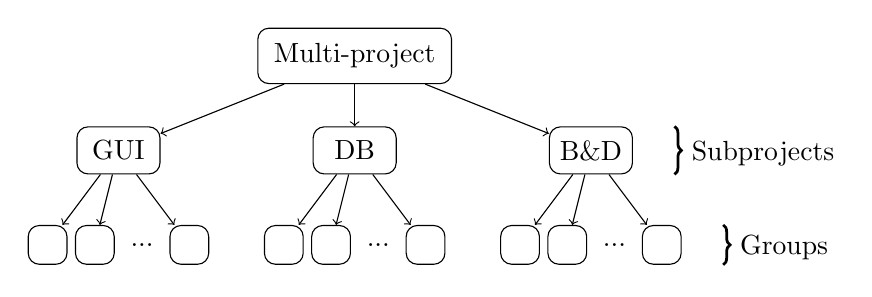
\begin{tikzpicture}[
  simple/.style={draw, rounded corners, minimum height=2em, minimum width=7em},
  simplefixed/.style={draw, rounded corners, minimum height=1.7em, minimum width=3em},
  square/.style={draw, rounded corners, minimum height=1.4em, minimum width=1.4em}]

  \node[simple] (mp) at (0,0) {Multi-project};

  \node[simplefixed] (gui) at (0,-1.2) {DB}; % NOTICE OTHER NAME THAN LABEL.
  \node[simplefixed] (db) at (-3,-1.2) {GUI};
  \node[simplefixed] (bd) at (3,-1.2) {B\&D};

  \node[square] (g1) at (-3.9, -2.4) {};
  \node[square] (g2) at (-3.3, -2.4) {};
  \node[] (g3) at (-2.7, -2.4) {...};
  \node[square] (g4) at (-2.1, -2.4) {};

  \node[square] (g5) at (-0.9, -2.4) {};
  \node[square] (g6) at (-0.3, -2.4) {};
  \node[] (g7) at (0.3, -2.4) {...};
  \node[square] (g8) at (0.9, -2.4) {};

  \node[square] (g9) at (2.1, -2.4) {};
  \node[square] (g10) at (2.7, -2.4) {};
  \node[] (g11) at (3.3, -2.4) {...};
  \node[square] (g12) at (3.9, -2.4) {};

  \draw[->] (mp) to (gui);
  \draw[->] (mp) to (db);
  \draw[->] (mp) to (bd);

  \draw[->] (db) to (g1);
  \draw[->] (db) to (g2);
  \draw[->] (db) to (g4);

  \draw[->] (gui) to (g5);
  \draw[->] (gui) to (g6);
  \draw[->] (gui) to (g8);

  \draw[->] (bd) to (g9);
  \draw[->] (bd) to (g10);
  \draw[->] (bd) to (g12);

  \draw[decorate, line width=1pt, decoration={brace, mirror}] ([xshift=1.5em]g12.south east) -- ([xshift=1.5em]g12.north east) node [midway, yshift=-0.1em, xshift=2.2em] {Groups};

  \draw[decorate, line width=1pt, decoration={brace, mirror}] ([xshift=1.5em]bd.south east) -- ([xshift=1.5em]bd.north east) node [midway, yshift=-0.1em, xshift=3.2em] {Subprojects};

\end{tikzpicture}
\caption{Illustration of multi-project organization}%
\label{fig:multi_project_organization}%
\end{figure}

\subsection{Work Products}
Two work products from Scrum are used, and every group is expected to help updating and maintaining these:

\begin{description}
  \item[Product Backlog] The product backlog contains the items of value to the customers, typically features, but also other items \parencite{larman2003}. On the multi-project level, there is a product backlog containing all items for the entire multi-project. The purpose of the multi-project level product backlog is to maintain the product backlog for the entire multi-project. The items in the product backlog are categorized according to each subproject. This enables each subproject to manage their items themselves, removing unnecessary management from the multi-project level.
  \item[Release Backlog] The release backlog contains the items that must be finished by the end of the current sprint \parencite{larman2003}. These items are selected from the product backlog during sprint planning meetings that each subproject hold.
\end{description}

Since it is not required for each group to use Scrum at the group level, there is no common sprint backlog.

The product backlog and release backlog contain the following items:

\begin{description}
  \item[Feature] Functional requirements (features) of the product are represented as user stories, as they are lightweight and fit well into the agile principles \parencite{rubin2012essential}.
  \item[Bug] Because bugs also represents behavior the user wants to be changed, they are considered no different from features \parencite{product-backlog2015}, and so are represented as user stories.
  \item[Constraint] A way of handling non-functional requirements, while not forcing it into a user story, is to turn the non-functional requirements into constraints \parencite[ch.16]{cohn2004}. Most often, these constraints are related to e.g.\ performance, usability, and security. Constraints can either be written on separate constraint cards \parencite[ch.16]{cohn2004}, or written in the corner of a user story card if it is relevant only to that single user story \parencite[ch.7]{cohn2004}. Due to the structure of multi-project, it makes sense for us to introduce two-level constraints. Multi-project constraints are relevant for the entire project as a whole, for example \emph{the software is written in Java} or \emph{all apps must be easy to internationalize}. Some constraints only apply to some areas of the project, and these are handled by the individual groups. Examples of these are \emph{the initial database sync must not take more than 5 minutes} or \emph{the user manager must only sync data of the user logged in}. These constraints are written on either a constraint card or on the relevant backlog item.
  \item[Knowledge Acquisition] Since no one in the multi-project has worked on it before, and because the project is complex, it is sometimes needed to investigate things to know it if is worth investing time in. Knowledge acquisition items can be formulated as user stories, but do not need to \cite{rubin2012essential}. Knowledge acquisition items are handled the same way as user stories. Estimation can be hard when investigating an unknown subject. The item can be investigated just enough to do further estimation by \emph{timeboxing} an initial investigation. This practice is in XP called a \emph{spike} \cite{cohn2004}.
  \item[Technical Work] Sometimes effort has to be spent on something the users are not directly interested in, e.g.\ updating software on the developer machines, updating the database software on a server, or refactoring parts of the code. These items can be part of the product backlog \cite{cohn2004}. They can also be formulated the same way as user stories \cite{rubin2012essential} and are handled the same way.
\end{description}

To summarize, the backlog items \emph{features} and \emph{bugs} are represented as user stories, whereas \emph{knowledge acquisition} and \emph{technical work} can be represented as user stories, but do not need to.

The following template, presented by \textcite{cohn2009}, is used for user stories in the multi-project:

$$\text{As a $\langle{}$\emph{type of user}$\rangle{}$, I want $\langle{}$\emph{some goal}$\rangle{}$ so that $\langle{}$\emph{some reason}$\rangle{}$}.$$

If the user story is suggested by developer, the source of the user story should be noted in case there are questions about it.

A user story must be sufficiently small for it to be completed in one sprint \parencite{cohn2009}. A user story must also have \emph{conditions of satisfaction}. These are high-level acceptance tests for the user story and must be true for the user story to be completed. A user story can have multiple conditions of satisfaction \cite{cohn2009}. Backlog items are prioritized by the product owner (possibly with help from the customers) \cite{larman2003}. An example of a user story can be seen in \figureref{fig:user_story_ex}. \todo{Nyt: eksempel på user story}

\begin{figure}
  \centering
  \begin{subfigure}[t]{0.47\textwidth}
    \centering
    \StickyNoteFront{\ECFAugie{} \large As a developer\\\\ I want monkey tests to run on the debug version of apps\\\\ so that they can be tested on a test database.}
    \caption{Front with user story}
  \end{subfigure}
  \begin{subfigure}[t]{0.47\textwidth}
    \centering
    \StickyNoteBack{\ECFAugie{} \large Monkey tests must run on debug APKs}
    \caption{Back with conditions of satisfaction}
  \end{subfigure}
  \caption{Example user story}\label{fig:user_story_ex}
\end{figure}

\subsection{Roles}
Two roles from Scrum are used in the multi-project:

\begin{description}
  \item[Scrum Master] \todo{Read this, it is revised} On the multi-project level, we are responsible for the development method. This means that we act as Scrum masters on the multi-project level. It is our role as Scrum masters to know and reinforce the sprint and project goals and visions and to ensure that the Scrum practices and values are followed on the multi-project level \cite{larman2003}. On the subproject level, one person is in charge of the meetings --- they make sure that the Scrum meetings on this level are held. On the group level, each group is free to do what they see fit.
  \item[Product Owner] The product owner (PO) is responsible for maintaining contact with the customers and being their representatives. It can be difficult to have a single PO with an external customer as customer in the multi-project. Therefore, the \bd and \db groups often do not have the external customer as their direct customer. Rather, these groups help the \gui groups achieve their goal by building solutions for them. The external customer is often not interested in the implementation details of build and database interfaces.

There are three POs in the multi-project, one for each subproject. The customer for the \gui PO is the external customer, whereas the customers for the \db and \bd POs are the groups of the other subprojects, as illustrated in \figureref{fig:po_illu}.
\end{description}

\begin{figure}%
\centering
\tikzsetnextfilename{po_illustration}
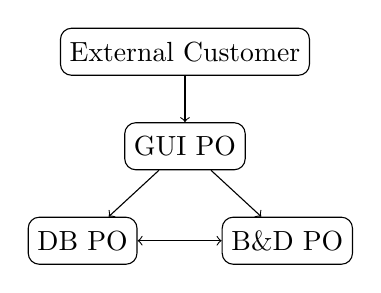
\begin{tikzpicture}[
  simple/.style={draw, rounded corners, minimum height=1.7em}]
  \node[simple] (extcust) at (0,1.2) {External Customer};
  \node[simple] (guipo) at (0,0) {GUI PO};
  \node[simple] (dbpo) at (-1.3,-1.2) {DB PO};
  \node[simple] (bdpo) at (1.3,-1.2) {B\&D PO};

  \draw[->] (guipo) to (dbpo);
  \draw[->] (guipo) to (bdpo);
  \draw[<->] (dbpo) to (bdpo);
  \draw[->] (extcust) to (guipo);

\end{tikzpicture}
\caption{Illustration of product owners}%
\label{fig:po_illu}%
\end{figure}

\subsection{Meetings}\label{sec:meetings}
Each week there is a meeting at the multi-project level. At this meeting the status of all groups in the multi-project is presented and the development method is evaluated. This ensures that all groups know the current status of the project. This meeting differs from a regular Scrum meeting in that it includes a point on method evaluation, so that the development method can be continually improved.

Each subproject holds internal Scrum meetings as well. These subproject Scrum meetings are held at least twice a week. The subprojects organize these meetings themselves and use them to discuss things that are relevant only for the members of the subproject.

Since there are three product owners in the multi-project, three sprint review meetings and three sprint planning meetings are held between sprints. These meetings were proposed by us, following the recommendation from \textcite{bird_davies_2007}, and afterward approved by the other groups.

\begin{description}
  \item[Sprint Planning Meetings]
  The purpose of the sprint planning meetings is to ensure that the product backlog is up to date and to select user stories for the release backlog.
  \begin{description}
    \item[GUI] At this sprint planning only one representative from each GUI group participate as \emph{pigs} (people who are allowed to talk), as well as the GUI PO and one representative from the other PO groups (although they have a less important role at this meeting). All other people in the multi-project are \emph{chickens} (people who are not allowed to talk). This meeting is held with the external customers. By making it so that primarily the \gui groups are pigs, the external customers are abstracted from internal development such as continuous integration and database management.
    \item[\db and \bd] There are separate sprint planning meetings for \db and \bd, where each subproject establishes the needs of the other subprojects. These meetings are internal, and the external customers do not participate, since \db and \bd do not have these as direct customers. \db and \bd will primarily have the GUI groups as their customers, who need various services from the \db and \bd subprojects, in order for them to fulfill their own backlog items directly related to the external customers. However, it might be that \db needs something from \bd and vice versa. Again, this abstracts the external customers from internal development.
  \end{description}
  \item[Sprint Review Meetings]
  At the sprint review meetings, the work done in the sprint is presented to the customers.
  \begin{description}
    \item[GUI] At this meeting the external customers are presented with the work of the GUI groups. Only the GUI groups participate as pigs at this meeting.
    \item[\db and \bd] \db and \bd each hold a separate sprint review meeting where they show the groups in the other subprojects what they have done in a sprint. The external customers are not present at these meetings, so that they are not bored with internal details. The \gui sprint planning meeting is separated from the \db and \bd sprint planning meeting by a few days, such that the product owners have time to organize, and make the requirements propagate from \gui to the other subprojects.
  \end{description}
  \item[Sprint Retrospective Meeting] \todo{Read this: this is new} The purpose of this meeting is to learn from the past to improve productivity in the future; a time for diagnosis of the multi-project \cite{scrumChecklist}. This meeting is held the Tuesday following a Sprint Review Meeting. In this meeting the previous sprint is discussed. There is extra focus on any problems regarding the development method during this meeting. Any concerns that are raised during this meeting are discussed, and possible solutions are suggested.
\end{description}

The sprint timeline is shown in \figureref{fig:gantt_dates}. Each sprint has approximately 8 full days per man. The exact sprint meeting dates are as follows:
\begin{itemize}
  \item Sprint 1
  \begin{itemize}
    \item \gui{}, \db{}, and \bd{} sprint planning meetings: February 15
    \item \gui{}, \db{}, and \bd{} sprint review meetings: March 10
  \end{itemize}
  \item Sprint 2
  \begin{itemize}
    \item Sprint 2 \gui{}, \db{}, and \bd{} planning meetings: March 12
    \item Sprint 2 \gui{}, \db{}, and \bd{} review meetings: April 8
  \end{itemize}
  \item Sprint 3
  \begin{itemize}
    \item Sprint 3 \gui{} planning meeting: April 8
    \item Sprint 3 \db{} and \bd{} planning meetings: April 15
    \item Sprint 3 \gui{}, \db{}, and \bd{} review meetings: April 27
  \end{itemize}
  \item Sprint 4
  \begin{itemize}
    \item Sprint 4 \gui{} planning meeting: April 27
    \item Sprint 4 \db{} and \bd{} planning meetings: May 4
    \item Sprint 4 \gui{}, \db{}, and \bd{} review meetings: May 20
  \end{itemize}
\end{itemize}
Notice that the \gui{} sprint planning meetings in the first two sprints are not separated from the \db{} and \bd{} planning meetings, as this delay was introduced after sprint 2.

\begin{figure}[ht]
  \centering
  \tikzsetnextfilename{gantt_dates}
  \begin{tikzpicture}
    \begin{ganttchart}[x unit=1mm, time slot format=isodate]{2015-02-10}{2015-05-30}
      \gantttitlecalendar{month=name}\\
      \ganttgroup{Sprint 1}{2015-02-15}{2015-03-10}\\
      \ganttgroup{Sprint 2}{2015-03-12}{2015-04-08}\\
      \ganttgroup{Sprint 3}{2015-04-15}{2015-04-27}\\
      \ganttgroup{Sprint 4}{2015-05-04}{2015-05-20}\\
      \ganttmilestone[milestone left shift=-0.9, milestone right shift=1.9]{Project Deadline}{2015-05-27}
    \end{ganttchart}
  \end{tikzpicture}
  \caption{\label{fig:gantt_dates} Gantt chart illustrating the sprint timeline}
\end{figure}

\subsection{Office Hours}
A vital part of working agile involves being able to easily communicate with all members of the multi-project. To ensure this all groups must be reachable on e-mail all weekdays 09:00--15:00, and preferably be in the group rooms. An exception for this is when there are courses.

\subsection{Tools}\label{sec:tools}
To support the development method of the multi-project, an online project management tool, Redmine \parencite{redmine-website}, is used. This tool was in use the previous year, and so this year the multi-project continues to use it. The main features are:

\begin{description}
  \item[Wiki] A wiki is used for various information, such as guides, how the development method is structured, meeting minutes, etc. Previous years had several separate wikis for each subproject. This year there is a single wiki providing central information.
  \item[Forum] The forum is used for non-crucial communication. It is mostly used for non-work related discussions such as social events. Groups are encouraged to communicate to each other directly by going to each other's group rooms, rather than using the forum.
\end{description}

In addition to Redmine, Google Docs is used by the POs to maintain the backlog.

\section{Software Development Method in Our Group}\label{sec:swmethod_ourgroup}
In our group we use Scrum as the development method, because it fits well into the multi-project development method. We have a Daily Scrum each morning where we summarize our work since last time and what we intend to do until the next Daily Scrum.

In addition to the previously described work products, we use a sprint backlog. After a sprint planning where backlog items have been selected by each group, we then split the backlog items selected by us into tasks and estimate those tasks using planning poker. Our unit of estimation is in half days, with the smallest unit being 1. This means that tasks that can actually be completed in less than a half day, may become overestimated. However, since there is an inherent imprecision in our estimations, this is not an issue. Our sprint backlog is physically placed on a wall, so that we can easily manage our tasks. In addition to the sprint backlog we use a burndown chart to measure our progress.

\todo{insert picture of wall}

\section{Group Roles in Multi-Project}\label{sec:multi_project_group_roles}
The multi-project contains responsibilities selected by groups within the multi-project. These roles include management of Redmine, server, Git, and Jenkins:

\begin{description}
  \item[Redmine General] Maintaining users, roles, and plugins on Redmine as well as managing work across the other Redmine groups below.
  \item[Redmine Wiki] Structuring and maintaining the wiki. They also read the content and make sure it is adequate, and notify the relevant groups if problems are found.
  \item[Redmine Forum] Structuring and moderating the forum.
  \item[Redmine Task Tracking] Structuring and maintaining the task tracker as well as helping people creating the items in the tracker. They also maintain guidelines for task creation.
  \item[Server] Maintaining the server software and controlling access to the server. They install and upgrade software upon request and help solving issues requiring root access.
  \item[Git] Maintaining the Git repositories and controlling access to these. Furthermore, they issue guidelines for Git usage.
  \item[Jenkins] Maintaining the Jenkins setup. This is the responsibility of our group, and as such will be detailed in this report.
  \item[Process] Supervising, developing, and refining the process method. This is also the responsibility of our group, and will as such also be detailed in this report.
  \item[Code Style] Developing and encouraging a code style across all code.
  \item[Customer Relations] Maintains customer relations. They review and send any email sent to the external customers.
  \item[Web Administrator] Maintains the public project website \url{http://giraf.cs.aau.dk}.
  \item[Android Guru] Persons with experience developing Android apps, and who can be asked for help.
  \item[Google Analytics and Google Play] Maintaining the Google Play listing of the software and generating guidelines for how to get crash reports from Google Analystics.
  \item[Graphics] Developing a graphical style and enforcing this as well as creating the graphics upon request.
\end{description}
\chapter{Software Configuration Management Plan}\label{chap:sw_intro_cm}
Software configuration management is an important part of any large software project. Configuration management can be defined as \emph{the discipline of identifying the configuration of a system at distinct points in time for the purpose of systematically controlling changes to the configuration and maintaining the integrity and traceability of the configuration throughout the system life cycle} \parencite[ch.6, p.6-1]{swebok}. The large size of the multi-project requires some form of software configuration management to handle and track the changes in the software. It can ease the workflow of developers and assure the quality of the product \parencite[ch.6]{swebok}. 

%\section{Software Configuration Management Plan}\label{sec:SCM_vision}
Our role as a group is to manage the development method, and therefore we have the responsibility of creating a Software Configuration Management Plan (SCMP). An SCMP specifies how items are controlled, by who, and by what tools \parencite[ch.6]{swebok}. The Guide to the Software Engineering Body of Knowledge (SWEBOK) \parencite[ch.6]{swebok} identifies some key areas of software configuration management.

This chapter describes how we plan and execute configuration management. We aim to make it as easy as possible for the developers, and therefore we will automate as much as possible.

\begin{chapterorganization}
  %\item in \sectionref{sec:SCM_vision} we identify a plan for the software configuration management and identify specific areas we want to improve or implement in the software configuration management practice;
  \item in \sectionref{sec:SCM_orgcontext} we \todo{\dummy};
  \item in \sectionref{sec:SCM_configitems} we \todo{\dummy};
  \item in \sectionref{sec:SCM_tools} we \todo{\dummy}.
\end{chapterorganization}

\section{Organizational Context}\label{sec:SCM_orgcontext}
In order to plan the software configuration management it is important to understand the organizational structure \parencite[ch.6]{swebok}. The multi-project has a quite unique structure. The development is performed and managed by students who work in small groups that each acts as a independent entity. While the product is being developed for the clients, the groups have other priorities than customer satisfaction. The work is being done for free, the motivation of the groups is to work on something interesting such that they can write a good report detailing the work and get a good grade. While we can suggest a process with specific procedures, we have no authority over the other groups. This means that the groups preferences weigh heavily when we select which software configuration management procedures to follow. In general, the feeling \todo{consensus?} in the groups are that the less formal communication and bureaucracy the better. This is reflected in the choice of Scrum as the basis for the project management, and will influence all of the decision regarding the software configuration management process planning and execution.

\section{Configuration Items}\label{sec:SCM_configitems}
A configuration item is a piece of software or a combination of hardware and software which is managed as a single entity \parencite[ch.6]{swebok}. Due to the desire of the groups to minimize overhead, there is no formal process which explicitly identifies the items that are to be controlled. The configuration items are identified by the groups of previous years, and by the groups during the project start up. New items might be discovered in the future, and they will be discussed at the multi-project status meetings and be described in the relevant sections in this report \todo{Tjek at vi gør dette}. The currently identified items and how they are managed are:

\begin{description}
  \item[Requirements] The requirements are managed by the subproject product owners as described in \sectionref{sec:project_overview}.
  \item[Built Application] The currently deployed version of all applications is controlled by the group responsible for Google Play. The current version of internally built applications are controlled by us through automatic building. When a change has been made to an application, it is re-built and all the unit tests are run.\todo{Kim fixed: What are these requirements, who sets these. please explain this.}. We ensure that the tests are run automatically, but it is the responsibility of the developers of each application to write the tests. The iOS applications developed on previous years are not under configuration management, as it was decided at the semester start that those applications will not be worked on.
  \item[Built Libraries] The binaries of all libraries are stored on a Maven repository. When a library builds successfully the binary is uploaded to the repository as a snapshot version. When the developers of the libraries decide that a new release should be made available, new versions of the libraries are uploaded. This way several versions of library binaries are stored.
  \item[Application and Library Source Code] The source code for the applications and libraries are controlled with Git \parencite{gitwebsite}. Each application and library has it own repository. The external dependencies are managed with Gradle which gets the correct version of each external library from Maven repositories. This ensures that we can control when to update the dependencies. Again, the source code for the iOS applications will not be managed.
  \item[Source Code Documentation] Documentation of source code is written by the developers of the software in Javadoc style. There is no formal process ensuring that it is actually written, and so it is solely up to the developers to do so. Documentation is, however, to be automatically generated.
  \item[The Supported Versions of the Android OS] Previous years selected the supported version of the Android OS to be API 15 and up. When new versions of the Android OS are released, they will be managed as well, and applications should be able to run on those versions.
  \item[The Supporting Tools Gradle and Android Studio] The developers on the multi-project use Android Studio as the main development tool for the Android applications. The version of Android Studio and Gradle are maintained by the \bd groups and any decision to upgrade is theirs. When the semester started the Android Studio and Gradle was upgraded. The Git group mainly handled this activity. We merged the upgrade from a different branch on Git to the master branch. The used version of Android Studio is 1.0.2 and 2.2.1 for Gradle.
\end{description}
We do not want to set up a change control board\parencite[p. 6-9]{swebok} (who can approve or reject change requests) since we use an agile development method. Setting up such a board would create unnecessary overhead and delay groups in doing their work.

\section{Tools}\label{sec:SCM_tools}
We use the following tools to manage the configuration items identified:

\begin{description}
  \item[Git] Git is used as the version control as mentioned previously. This was set up by previous years, and we continue to use their setup. \group{8} manages Git.
  \item[Jenkins] Jenkins is used to automatically build and test applications. Jenkins is detailed in \sectionref{sec:jenkins}. Jenkins is used for all applications throughout the multi-project, except for the iOS applications. We manage Jenkins.
  \item[Artifactory] The Artifactory tool is a Maven repository that stores various versions of binaries of the libraries in the multi-project. \todo{Ref til hvor Artifactory bliver beskrevet i detajler}
  \item[Doxygen] We use Doxygen to generate source code documentation. The use of Doxygen is described further in \sectionref{sec:automated_documentation_gen}. Doxygen is managed by us, but the documentation itself is managed by the developers and \group{5} who issue guidelines on the documentation.
\end{description}

% Sprints
\clearpage{}
\ihead{Sprint \arabic{sprintcounter}} % Puts >>Sprint X<< in headers.

\sprint{Initialization Phase and Configuration Management}
% Chapters
\chapter{Sprint Planning}\label{chap:s4_sprintplanning}

\begin{chapterorganization}
  \item in \sectionref{sec:S4_bd} we describe the user stories we commit ourselves to during the \bd sprint planning meeting.
  \item in \sectionref{sec:S4_group} we describe the sprint planning in our group and lists our tasks with reference to a user story.
\end{chapterorganization}

\section{\bdtitle Sprint Planning}\label{sec:S4_bd}
During the \bd sprint planning we choose to work on the following user stories in this sprint. They are labeled with a number in parentheses for reference.

\todo{Tilføj conditions of satisfaction}

\begin{description}
  \item[Job Prioritization on Jenkins (1)] Developers have specified a desire for some jobs to have a higher priority than other jobs. For example developers would like libraries to run before apps.
  \item[Monkey Test on Debug Versions of Apps (2)] With the \db groups working on implementing database sync, they are making a test database available. Monkey tests currently use a development database that might be wiped accidentally. To ensure this does not happen monkey tests should run on debug APKs rather than release APKs.
  \item[Decrease Build Times on Jenkins Further (3)] When the queue on Jenkins is long, jobs can take a very long time to build. As we discussed in \sectionref{sec:non-emulator_testing}, the build times can be further reduces by working on the emulator.
  \item[Easy Download and Installation of all Apps (4)] In the previous sprint developers were not always using the latest versions of all apps, which lead to issues at the sprint end. The developers therefore want an easy way to download and install the newest version of all apps on their devices.
  \item[Document Jenkins Structure for Next Semester (5)] To make it easy for the next semester to start working with Jenkins, documentation of the Jenkins structure used is needed.
\end{description}

\section{Group Sprint Planning}\label{sec:S4_group}
At our internal sprint planning we divide the chosen user stories into tasks and estimate them. For this sprint, we have a total of 70 half days of work. \tableref{tab:sprint4_tasks} shows the tasks we have committed to solve for this sprint. Tasks with a plus (+) are tasks that have been added during the sprint as they were discovered.

\begin{table}%
  \centering
  \begin{tabular}{p{0.6\textwidth}rr}
    \toprule
    \textbf{Task} & \textbf{User Story} & \textbf{Estimation} \\
    \midrule
    Investigate conditions of satisfaction for our user stories & na & 2 \\
    Make a program to download and install the newest version of each app & 4 & 2 \\
    Make it so that the Android emulator is only started when no other devices are connected & 3 & 6 \\
    Connect to all Android devices wirelessly & 3 & 2 \\
    Connect Android devices permanently to the Internet & 3 & 2 \\
    Put debug APKs onto the ftp & 2 & 1 \\
    Make monkey tests use debug APKs & 2 & 1 \\
    Install Jenkins Prioritization Plugin & 1 & 1 \\
    Choose schedule for prioritization plugin & 1 & 2 \\
    Identify areas for Jenkins documentation (spike) & 5 & 2 \\
    Write about Jenkins files on server (from spike) & 5 & 2 \\
    Write about Jenkins structure (from spike) & 5 & 2 \\
    Investigate method to decrease emulator usage time (spike) & 3 & 1 \\
    % \midrule
    % \textbf{Down-prioritized tasks} & & \\
    % \midrule
    % \midrule
    % \textbf{Missed tasks} & & \\
    % \midrule
    % \textbf{Rejected tasks} & & \\
    % \midrule
    \midrule
    \textbf{Original total} & & y \\
    \textbf{Total} & & x \\
    \bottomrule
  \end{tabular}
\caption[Sprint 4 backlog]{Sprint backlog for sprint 4, excluding report tasks. The tasks are listed in no particular order.}
\label{tab:sprint4_tasks}
\end{table}

\todo{Tasken ``Investigate method to decrease emulator usage time (spike)''har vi ikke, men lavede uformelt den første dag da vi lavede sprint planning i gruppen}

\todo{I dette sprint skal vi også skrive frontmatter, backmatter, introduktion og konklusion}
%!TEX root = ../report.tex
\chapter{Setting Up Automated Build}\label{chap:config_management}
Starting the first sprint we need to understand the systems given to us by previous semesters. We mainly look at setting up automated build, but also do some setup of the Redmine tool.

\begin{chapterorganization}
  \item in \sectionref{sec:redmine-conf} we describe how we customize Redmine to suit our needs;
  \item in \sectionref{sec:jenkins} we describe the platform for continuous integration, Jenkins, that we use in the project;
  \item in \sectionref{sec:build_automation} we explain how we set up automation of the builds and discuss version control branching strategies as well as automated testing and lint checking;
  \item in \sectionref{sec:automated_documentation_gen} we explain how we set up automated documentation generation.
\end{chapterorganization}

\section{Configuring Redmine}\label{sec:redmine-conf}
The developers of last year used Redmine for various project management functions. We need to evaluate which functions to keep.
One of these functions is an issue tracker. We choose to keep it, but not as a traditional issue tracker.  Instead we customize it so that it contains the product backlog and release backlog.  This setup is not ideal as it can be hard to manage at times, but it is what the multi-project has available without much more needed effort. We collaborated with \group{3} (Redmine general) and \group{10}. We specified how user stories should be handled in Redmine, and \group{3} and \group{10} implemented the changes.

Also, a Gantt chart feature had been installed by previous years. The Scrum method does not advocate Gantt charts or other dependency charts \parencite{larman2003}. As such, we collaborated with \group{3} to remove this from Redmine. The other unused features have not been removed, since it was deemed unnecessary to spend time on doing so.

Redmine also contains other features such as a roadmap, burndown charts, and news. While these features are present on the main page, they are not used. The burndown chart in particularly is not used since no common sprint backlog is used, and as such the burndown chart cannot be used at the multi-project level.

\section{Jenkins: Continuous Integration Platform}\label{sec:jenkins}
An open source tool for continuous integration, Jenkins \parencite{JenkinsWebsite}, was used by previous years. We will use this as our continuous integration platform. It supports source control management tools such as Git \parencite{gitwebsite}, as well as build automation tools such as Maven \parencite{mavenwebsite}. It is extensible via numerous available plugins. Jenkins allows for a sophisticated continuous integration setup, however the setup by previous years is rather basic and we want to improve it in several ways.

\subsection{Upgrading Jenkins and Plugins}
We inherited the old installation which had not been updated in a long time. Jenkins itself and all the Jenkins plugins had updates available. We updated everything to the newest versions.

\subsection{Setting up Roles in Jenkins}
The inherited Jenkins installation was open to anybody. We do not find this sensible as we need to control the build process. Allowing everybody access will likely end in someone modifying a setting without our knowledge. Because we set up a mechanism for automatic build, other people do not need the option to start builds manually. It might even interfere with the automatic build, if other people have access to the Jenkins configuration.

It is important that everyone can see the build process, however. According to Martin Fowler, it is important that everyone is able to see the state of builds and which parts of the overall system that are currently worked on \parencite{fowlerCI}. In addition to this, we find it important that developers can follow the testing process of their new code, and how stable different projects are. This way, we are able to transfer human resources between projects if needed, and it may work as a motivation for the developers to create stable builds. Because of this, we give developers read-only access to Jenkins, while we are the only people with write access.
\kimnote{What is a project in this context. I am guessing that is not the multi-project that you are talking about. Please make your terminology very clear or use another word. A project can be several things, the role of a group,a student project, or a maven project.}

\section{Build and Test Automation}\label{sec:build_automation}
The inherited project has no build automation. As a part of the automated build and deployment story, we want to be able to build the code automatically, and even continuously. We decide to set it up in two stages. In the first stage we schedule all jobs to run nightly. This gives us some level of build automation and gives us time to investigate merge strategies and set it up properly. The nightly job is set to run every day at midnight.

\subsection{Merge Strategy}\label{sec:branching_strategy}

\begin{figure}
\begin{subfigure}[b]{\linewidth}
\centering
\tikzsetnextfilename{mergestrategy}
\begin{tikzpicture}
% MASTER
\node[text width=2cm] at (0,1) {\mono{master}};
\node(master_a) [draw, circle, minimum size=0.5cm] at (2,1) {\mono{A}};
\node(master_head) [draw, circle, minimum size=0.5cm] at (5,1) {\mono{D}};
\node(master_head_label) [] at (5,2) {\mono{HEAD}};
\draw[->, >=latex] (master_head) -- (master_a);
\draw[->, >=latex] (master_head_label) -- (master_head);

% LOCAL
\node[text width=2cm] at (0,0) {\mono{dev\_branch}};
\node(local_b) [draw, circle, minimum size=0.5cm] at (3,0) {\mono{B}};
\node(local_c) [draw, circle, minimum size=0.5cm] at (4,0) {\mono{C}};
\draw[->,>=latex] (local_b) -- (master_a);
\draw[->,>=latex] (master_head) -- (local_c);
\draw[->,>=latex] (local_c) -- (local_b);
\begin{pgfonlayer}{background}
  \filldraw [line width=4mm,join=round,black!10]
      (-1, 1.2)  rectangle (6,0.8)
      (-1, 0.2)  rectangle (6,-0.2);
\end{pgfonlayer}
\end{tikzpicture}
\caption{The direct commit strategy}\label{fig:commit_stratagy_a}
\end{subfigure}\\
\begin{subfigure}[b]{\linewidth}
\centering
\begin{tikzpicture}
% MASTER
\node[text width=2cm] at (0,2) {\mono{master}};
\node(master_a) [draw, circle, minimum size=0.7cm] at (2,2) {\mono{A}};
\node(master_head) [draw, circle, minimum size=0.7cm] at (6,2) {\mono{D}};
\node(master_head_label) [] at (6,3) {\mono{HEAD}};
\draw[->, >=latex] (master_head) -- (master_a);
\draw[->, >=latex] (master_head_label) -- (master_head);

% PENDING HEAD
\node[text width=2cm] at (0,1) {\mono{intermediate}};
\node(ph_head) [draw, circle, minimum size=0.7cm] at (5,1) {\emph{\mono{I}}};
\draw[->, >=latex] (master_head) -- (ph_head);

% LOCAL
\node[text width=2cm] at (0,0) {\mono{dev\_branch}};
\node(local_b) [draw, circle, minimum size=0.7cm] at (3,0) {\mono{B}};
\node(local_c) [draw, circle, minimum size=0.7cm] at (4,0) {\mono{C}};
\draw[->,>=latex] (local_b) -- (master_a);
\draw[->,>=latex] (ph_head) -- (local_c);
\draw[->,>=latex] (local_c) -- (local_b);

\begin{pgfonlayer}{background}
  \filldraw [line width=4mm,join=round,black!10]
      (-1, 2.2)  rectangle (7,1.8)
      (-1, 0.2)  rectangle (7,-0.2);
  \filldraw [line width=4mm,join=round,black!10]
      (-1, 1.2)  rectangle (7,0.8);
\end{pgfonlayer}
\end{tikzpicture}
\caption{The pre-tested commit strategy}\label{fig:commit_stratagy_b}
\end{subfigure}
\caption[Different branching strategies]{Different branching strategies. A circles represents a commit and an arrow represents a reference to a commit.}\label{fig:commit_stratagy}
\end{figure}

As the name \emph{continuous integration} suggests, code should be integrated into the mainline (or \emph{master branch}) of the project frequently \parencite{fowlerCI}. According to Martin Fowler, frequent merges ensure that merges generally will be small and easy to perform \parencite{fowlerFeatureBranch}. The master branch must be stable and always in a release-ready state. If it breaks, it should be the team's first priority to fix it. A consequence of this is that the whole team is affected when a developer introduces an error, which has a negative influence on the overall productivity.

We assess two strategies to accommodate these consequences of continuous integration\kimnote{sounds awesome, insert citations! :)}: a \emph{direct commit strategy} and the \emph{pre-tested commit strategy}. In the direct commit strategy, every developer integrates its code directly to the master branch. It is the developer's own responsibility that the code works. This is the simplest, and one may say, the most agile way of integrating code with the master branch. An illustration of the direct commit strategy can be seen in \figureref{fig:commit_stratagy_a}. A developer creates a branch from the master branch and develops their code (commits \mono{B} and \mono{C}) on this before merging it directly into the master branch (commit \mono{D}).

An alternative to integrating code directly with the master branch is to use pre-tested commits \parencite{fowlerPendingHead}. A pre-tested commit uses a special branch which is an intermediate place for building and testing code before it is merged into the master branch. The code will only be merged into the master branch if it passes the tests. This ensures that the master branch will always work, but the merging workflow will be more complex as the developer must pull from one branch and push to another. The strategy is illustrated in \figureref{fig:commit_stratagy_b}. The developer creates a branch from the master branch and develops its code on here. When completed, the code is merged with the intermediate branch (commit \emph{\mono{I}}), which will build and test the code before eventually merging it with the master branch (commit \mono{D}).

For the first sprint, we choose to implement the direct commit strategy, primarily because of its simplicity. It is important to get continuous integration up running so the developers can start to develop code, and it would be too costly to spend time implementing a pre-tested commit strategy as this will block the progress of all other developers. We are unsure about how the developers handle the increased responsibility, so in the preparation of the second sprint, we will evaluate this strategy and consider whether we should implement the pre-tested commit strategy instead. \kimnote{Remember to evaluate the strategy.}

We implement this by setting up a post-receive hook that invokes Jenkins to automatically build any project that pulls from the repository that receives a push\kimnote{Punctuation is needed, I am a bit unsure of what is meant in the sentence.}. The hook can be seen in \listingref{lst:hook_script_first}. \mono{curl} sends to Jenkins the needed information for starting a build on a job associated with a particular repository. \mono{http://cs-cust06-int.cs.aau.dk/git-ro/\$(basename \$(pwd))} is the link for the repository to update. Since the script is stored in only one place, and there are several repositories, the name of the repository that invokes the hook is found by \mono{\$(basename \$(pwd))}. Finally a message is displayed to the user that pushed to tell them that Jenkins will start building.\todo{Nyt: LÆS}

\begin{lstlisting}[language=bash,showstringspaces=false,caption=Git hook script,label=lst:hook_script_first]
curl -s http://localhost/jenkins/git/notifyCommit?url= http://cs-cust06-int.cs.aau.dk/git-ro/$(basename $(pwd)) > /dev/null

echo "Thank you for your push. Jenkins will be serving you in a moment."
\end{lstlisting}

\subsection{Continuous Build}
The output of a build is an APK file, which is a package format used to distribute and install software onto Android. These files need to be signed before they can be installed. As such, we add a post-build task to Jenkins which signs and verifies the APK files as well as moves it into a common APK folder for all projects.

After deciding upon the merge strategies, we improve the nightly build and test automation. Instead of building and testing nightly, we automatically build and test projects whenever new code is pushed to the master branch. This gives the developer fast feedback on the integration of the code, and we are likely to discover an error in the code faster than before. The automatic build is triggered by a git-hook on each repository which is a way to execute a script when specific git events occur. The script is executed whenever something is pushed to the repository. It sends an HTTP request to the Jenkins server which triggers builds of all projects that depend on the repository.

\subsection{Continuous Deployment}
\label{sec:auto_deploy}
When we have built a project we would also like to deploy it. This was not a part of the sprint initially, but UI testing is dependent on the output of the deployment. On Jenkins there is a project called \emph{deployment} which builds all other projects, signs (only some of) them and moves them to the aforementioned directory. We remove this project and make it a part of the build process of every project to do this themselves, and ensure there are no redundant APKs present in the APK directory. By making it a part of every project we also ensure that there always is an up-to-date version of all applications whenever they pass a build, complementing our vision for continuous integration. This additional work was unplanned, and we do not have time to set it up on all projects in this sprint.


\subsection{Continuous Test}
\label{sec:test_automation}
Now that the automatic test setup is created, we examine the different types of automatic tests we can use on Android.

Because one of the ideas behind automated build is to give the developer fast feedback on the state of the code, the build and test process should be fast. The Extreme Programming (XP) development method states 10 minutes as a guideline for how long time a build should take \parencite{beck2004}. While we think this is a reasonable time, not all parts of the system can be thoroughly tested in that time. In such cases, Martin Fowler suggests that the fastest and general tests should be whenever a commit is pushed to the master branch, and slower tests can be triggered for later execution \parencite{fowlerCI}. We call these kinds of tests \emph{delayed tests}.

\subsubsection{Unit Testing}
During the initial investigation of the inherited code base we found some existing unit tests in one of the Giraf projects. These tests utilize the Android unit testing framework included in the Android framework \parencite{AndroidUnit}. The unit tests runs in an emulated Android environment, or on actual Android devices if any are connected to the computer. We therefore decide to postpone any further investigation into unit testing frameworks. Instead, we focus on getting the existing unit tests to run, both locally and in Jenkins. The tests were immediately runnable through Android Studio 0.4.6. However, Android Studio does something behind the scenes when it runs the tests, and therefore we could not run them from the command line, which means that we cannot run them in Jenkins. However, the most recent Android studio, version 1.0.2, uses Gradle exclusively to run the tests. This means that when the projects are migrated to the new version, we are able to run the tests with Jenkins.
The other projects did not have any tests, so we create test projects, with examples of tests to verify that Jenkins can run the tests. In addition it makes it easy for the other groups to start testing, as there is then a unit testing framework in place, as well as an example test. Groups are then encouraged to write tests for their code, but not obliged.

Currently, Jenkins starts a new emulator before each project is built. This adds a significant delay to the build. The build time for the entire app has increased from 20 to 90 minutes. This is unfortunate, but for now we won't spend more time improving on this. We may return to this in a later sprint. Unit tests are the simplest tests we have, and we do not want these to be handled as delayed tests.
\kimnote{Remember to follow up on this.}

\subsubsection{UI Testing and Monkey Testing}
Because Android applications contain a graphical user interface, it is not sufficient to only test the backend libraries. On the overall level, there are two ways of performing automatic testing of the user interface in Android: UI tests and monkey tests. UI tests is a way of declaring specific sequences of events and their expected behaviors. For example, a test may specify a click on a settings button and assert that this actually opens the settings activity. Writing UI tests can be labor intensive, though, and the maintenance of the tests can get quite comprehensive. As an alternative, monkey testing can be used. Monkey testing is a test performed by inputting a random sequence of events, such as buttons clicks and touches, into a device. That way, the user interface of an app is randomly tested. There are no guarantees that all parts of the app will be tested, but the setup of the test is very simple. The official Android SDK has monkey testing facilities built in, and there exists a Jenkins plugin for running these. Because of the simplicity of monkey testing, and because the GUI application developers have requested this as a tool for discovering bugs in the code, this is the way we automatically test the user interface. We plan to run monkey tests on Jenkins during the night, as delayed tests, when the server is otherwise idle. The developers will get notified if issues are found.

While the Android monkey tool can test multiple applications at once, the Jenkins plugin does not support that feature. The monkey test command can take as an argument a number of packages (apps) to test, using the \mono{-p} option, for example \code{monkey -p package1 -p package2 -p package3 5000}. The Jenkins plugin does not support making more than one \mono{-p} option. The plugin is open source, so we add support for this feature, by contributing code\footnote{Commits on Github (\url{https://github.com/jenkinsci/android-emulator-plugin}): \href{https://github.com/jenkinsci/android-emulator-plugin/commit/71385cfb3e3bb4dfa6d11170c52ee69808a4f72f}{71385cf},  \href{https://github.com/jenkinsci/android-emulator-plugin/commit/811bfac657565b25ce2f7fc9d6399d9f22bb6042}{811bfac}, \href{https://github.com/jenkinsci/android-emulator-plugin/commit/5395bb1fd23032cab48a7bfff61a26544f078785}{5395bb1}}. Multiple packages are delimited by comma. The reason for this is that we found that some users exploited the way the package name was inserted as an argument to the monkey tool in order to insert different arguments. Because a comma character is not used in any argument to the monkey tool (compared to for example a whitespace character), we expect that no existing users will be influenced by the change.
\kimnote{You could add the code you contributed, only do it if you think it is interestingly to look at.}

Additionally the plugin requires the installation of the apps to test. The continuous deployment task, was not finished, so there are no APKs available for the monkey tester. Therefore the automatic UI testing could not be completely set up and ready in this sprint.

\subsubsection{Concolic Testing}
Concolic testing is a way to statically analyze code in order to find bugs, e.g.\ potential null pointer exceptions. Concolic testing uses a combination of symbolic execution and testing of particular paths in order to maximize code coverage \parencite{concolic_testing_2015}.

To our knowledge, the only framework for concolic testing that works with Android projects is \emph{Acteve} \parencite{AnandNHY12, AnandH11}. The documentation for this framework is non-existent, and we cannot find anything except for an unsuccessful attempt to build and run Acteve \parencite{chenxiong-acteve}.

We already have unit testing and many crash reports to occupy the time of many multi-project groups, and as such we do not think concolic testing is worth the payoff, so we will not spend more time investigating this.

\subsection{Automated Lint Check}\label{sec:automated_lint}
Lint checking is static code analysis that scans the source code for potential bugs and improvements. We investigate the possibility of automating lint checks on the source code, as we suspect this will uncover a wide range of improvements.

An official tool, Android Lint \parencite{AndroidLint}, for linting Android project source files exists. It checks for potential bugs and optimization improvements for correctness, security, performance, usability, accessibility, and internationalization.

There are some important considerations to consider before linting the source code automatically. The code base is inherited from earlier years and no lint checking to our knowledge was performed on this. Linting the code will produce a considerable amount of warnings. It is therefore not possible for us to let a build fail if it contain any warnings.

In this first sprint, we set up automating the lint check in Jenkins to be performed on all builds. The warnings are presented in the build overview screen, as seen in \figureref{fig:jenkins-overview}, and we hope that having a low number of lint warnings will be incentive enough for each group to fix warnings.

\begin{figure}[htbp]
    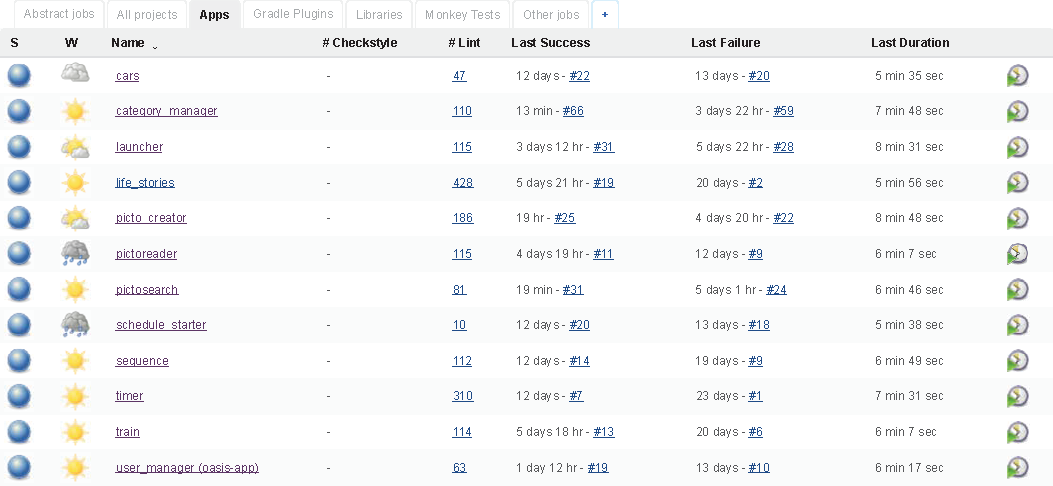
\includegraphics[width=\textwidth]{graphics/jenkins-overview.pdf}
    \caption{Screenshot of a section of the build overview screen, which shows the lint warning column}
    \label{fig:jenkins-overview}
\end{figure}

Over time, we hope that the presence of serious lint warnings can be a reason to fail a build. We may adopt this practice in a later sprint, and to help speed up this adoption we may set it up as follows. As there are a large number of lint warnings already in the code, we will select a baseline day. Groups will not be \emph{punished} (i.e.\ the build fails) for lint warnings that were present before the baseline day. Only newly introduced lint warnings will be considered and punished. Fixing old lint warnings from before the baseline day will of course count positively.
\kimnote{Remember to evaluate this later.}

\section{Automated Documentation Generation}\label{sec:automated_documentation_gen}
When working with a large code base, people will most likely not have insight in all parts of the code. Some kind of documentation is helpful in order to know how to use libraries. However the agile manifesto states that one should prioritize working code over documentation \parencite{agile-manifesto-web}. Therefore we do not intend to write comprehensible documentation of the code. A consequence of being agile is that the system architecture is likely to change rapidly --- so it is important that little effort is required for updating the documentation. To make the documentation easy to find, we want the documentation for all projects accessible from one place. Based on these requirements, we choose to use a documentation generator which automatically generates documentation from the code rather than writing such documentation manually. The documentation will not be all-encompassing, but act more like a guide to the code.

We investigate the Javadoc \parencite{javadoc} and Doxygen \parencite{doxygen} tools. Both tools are cross-platform and can be integrated with Jenkins. Javadoc can generate documentation in HTML and Doxygen can generate both HTML and \LaTeX. We will generate HTML documentation which will be hosted on our server.

Javadoc is the official documentation generator for Java and generates documentation based on specially formatted comments embedded in the source code. This format is integrated in Android Studio, making the documentation easily accessible where needed. In addition, parts of the existing code already contain Javadoc comments. A problem with Javadoc, however, is that it follows the packages and classes referred in a Java file. A requirement for this is that the source code must be a correctly structured Java project in order for the tool to find the different classes. This makes it complicated to comply with the requirement of having documentation of all projects in one place, because a combination of all projects may not form a valid Java project. The source code of all projects cannot simply be copied into one directory and fed to the Javadoc tool.

The Doxygen tool is a cross-language documentation generator that supports the same documentation syntax as Javadoc. Doxygen does not follow the class dependencies but simply parses the specified files. The HTML-documentation is very similar to that of Javadoc, and because it is more convenient to use, we have chosen to use this tool for documentation generation.\todo{Lav evt. diagram der viser hvordan filer bliver samlet og en dokumentation bliver lavet og smidt på en side}

\subsection{Documentation Generation in Jenkins}
We have configured a Jenkins job to generate the documentation for all projects. This job pulls the most recent state of the master branch of each project and executes the Doxygen tool on all code. On the current code base, the doxygen tool uses 3--7 minutes to generate the documentation because of the size of it. Because we do not want to block more important jobs, such as building and testing new commits, we choose to run this job nightly.
\chapter{Sprint End}\label{chap:sprint1_end}
Write about how the sprint end went.

\section{Sprint Goals}
\todo{What did we manage to make. Compare with our release backlog as mentioned in the sprint planning chapter}

\section{Process Evaluation During Sprint}
\todo{Write about process evaluation stuff we did during sprint. In particular how we investigated the having three pos and why we did so}

\section{Sprint Meetings}
\todo{Major sprint meetings of the sprint where we were involved.}

\subsection{GUI Sprint End}
\todo{What happened here?}
\todo{Shall we briefly mention that we did some (although minor) work at the gui sprint planning}

\subsection{\bd Sprint End}
\todo{What happened here? In particular what did our group show?}

\subsection{\db Sprint Planning}
\todo{We were headhunted to assist in this meeting, due to difficulties.}

\section{Multi-Project Sprint Review}
\todo{Girafmøde 17--03}
\todo{Mere tid mellem GUI sprint planning og de resterende sprint planning for at tillade GUI grupper mere tid til at sætte sig ind i deres release backlog}

\sprint{Improving Automation}
\chapter{First chapter in this}%\label{chap:...}
Chapter description

% Chapters
\chapter{Sprint Planning}\label{chap:s4_sprintplanning}

\begin{chapterorganization}
  \item in \sectionref{sec:S4_bd} we describe the user stories we commit ourselves to during the \bd sprint planning meeting.
  \item in \sectionref{sec:S4_group} we describe the sprint planning in our group and lists our tasks with reference to a user story.
\end{chapterorganization}

\section{\bdtitle Sprint Planning}\label{sec:S4_bd}
During the \bd sprint planning we choose to work on the following user stories in this sprint. They are labeled with a number in parentheses for reference.

\todo{Tilføj conditions of satisfaction}

\begin{description}
  \item[Job Prioritization on Jenkins (1)] Developers have specified a desire for some jobs to have a higher priority than other jobs. For example developers would like libraries to run before apps.
  \item[Monkey Test on Debug Versions of Apps (2)] With the \db groups working on implementing database sync, they are making a test database available. Monkey tests currently use a development database that might be wiped accidentally. To ensure this does not happen monkey tests should run on debug APKs rather than release APKs.
  \item[Decrease Build Times on Jenkins Further (3)] When the queue on Jenkins is long, jobs can take a very long time to build. As we discussed in \sectionref{sec:non-emulator_testing}, the build times can be further reduces by working on the emulator.
  \item[Easy Download and Installation of all Apps (4)] In the previous sprint developers were not always using the latest versions of all apps, which lead to issues at the sprint end. The developers therefore want an easy way to download and install the newest version of all apps on their devices.
  \item[Document Jenkins Structure for Next Semester (5)] To make it easy for the next semester to start working with Jenkins, documentation of the Jenkins structure used is needed.
\end{description}

\section{Group Sprint Planning}\label{sec:S4_group}
At our internal sprint planning we divide the chosen user stories into tasks and estimate them. For this sprint, we have a total of 70 half days of work. \tableref{tab:sprint4_tasks} shows the tasks we have committed to solve for this sprint. Tasks with a plus (+) are tasks that have been added during the sprint as they were discovered.

\begin{table}%
  \centering
  \begin{tabular}{p{0.6\textwidth}rr}
    \toprule
    \textbf{Task} & \textbf{User Story} & \textbf{Estimation} \\
    \midrule
    Investigate conditions of satisfaction for our user stories & na & 2 \\
    Make a program to download and install the newest version of each app & 4 & 2 \\
    Make it so that the Android emulator is only started when no other devices are connected & 3 & 6 \\
    Connect to all Android devices wirelessly & 3 & 2 \\
    Connect Android devices permanently to the Internet & 3 & 2 \\
    Put debug APKs onto the ftp & 2 & 1 \\
    Make monkey tests use debug APKs & 2 & 1 \\
    Install Jenkins Prioritization Plugin & 1 & 1 \\
    Choose schedule for prioritization plugin & 1 & 2 \\
    Identify areas for Jenkins documentation (spike) & 5 & 2 \\
    Write about Jenkins files on server (from spike) & 5 & 2 \\
    Write about Jenkins structure (from spike) & 5 & 2 \\
    Investigate method to decrease emulator usage time (spike) & 3 & 1 \\
    % \midrule
    % \textbf{Down-prioritized tasks} & & \\
    % \midrule
    % \midrule
    % \textbf{Missed tasks} & & \\
    % \midrule
    % \textbf{Rejected tasks} & & \\
    % \midrule
    \midrule
    \textbf{Original total} & & y \\
    \textbf{Total} & & x \\
    \bottomrule
  \end{tabular}
\caption[Sprint 4 backlog]{Sprint backlog for sprint 4, excluding report tasks. The tasks are listed in no particular order.}
\label{tab:sprint4_tasks}
\end{table}

\todo{Tasken ``Investigate method to decrease emulator usage time (spike)''har vi ikke, men lavede uformelt den første dag da vi lavede sprint planning i gruppen}

\todo{I dette sprint skal vi også skrive frontmatter, backmatter, introduktion og konklusion}

\chapter{Some Chapter}
\section{Improving Build Times}

To identify in which parts of the build process to make faster, we measure the time different parts of the Launcher project take. The Launcher project is the main application which depends on many other subprojects. The timings are measured on the Jenkins server and shown in \figureref{fig:launcher_build_times}. The shows the build timings of the Launcher application and the different subprojects (\emph{Oasis-lib, Giraf-Component, Local-db, Barcode-scanner, and Metadata}), as well as the startup time for the emulator.\todo{Kan vi regne med, at submoduler bliver binære filer?}

\begin{figure}
%\begin{tikzpicture}
%  \begin{axis}[xbar stacked,
%axis y line*= none, axis x line*= bottom,
%xmajorgrids = true,
%ytick = data,
%yticklabels = {},
%tick align = outside,
%xtick pos = left,
%bar width=6mm,
%y=8mm,
%nodes near coords,
%legend style={
%  legend columns=-1,
%  anchor=north,
%  draw=none,
%},
%area legend,]
%    \addplot coordinates
%    {(209,0)};
%    \addlegendentry{Metadata}
%    \addplot coordinates
%    {(6625,0)};
%    \addlegendentry{Barcode-scanner}
%    \addplot coordinates
%    {(8393,0)};
%    \addlegendentry{Launcher}
%    \addplot coordinates
%    {(17223,0)};
%    \addlegendentry{Local-db}
%    \addplot coordinates
%    {(18000,0)};
%    \addlegendentry{Emulator}
%    \addplot coordinates
%    {(104696,0)};
%    \addlegendentry{Giraf-component}
%    \addplot coordinates
%    {(159497,0)};
%    \addlegendentry{Oasis-lib}
%  \end{axis}
%\end{tikzpicture}
\caption{Timings during build of the Launcher project.}\label{fig:launcher_build_times}
\end{figure}

\sprint{Process Improvements and Monkey Testing}
\part{Sprint 3}

\chapter{First chapter in this}%\label{chap:...}
Chapter description

% Chapters
%\input{part_spring1/somefile}

\sprint{Some title}

\chapter{Sprint Planning}\label{chap:s4_sprintplanning}

\begin{chapterorganization}
  \item in \sectionref{sec:S4_bd} we describe the user stories we commit ourselves to during the \bd sprint planning meeting.
  \item in \sectionref{sec:S4_group} we describe the sprint planning in our group and lists our tasks with reference to a user story.
\end{chapterorganization}

\section{\bdtitle Sprint Planning}\label{sec:S4_bd}
During the \bd sprint planning we choose to work on the following user stories in this sprint. They are labeled with a number in parentheses for reference.

\todo{Tilføj conditions of satisfaction}

\begin{description}
  \item[Job Prioritization on Jenkins (1)] Developers have specified a desire for some jobs to have a higher priority than other jobs. For example developers would like libraries to run before apps.
  \item[Monkey Test on Debug Versions of Apps (2)] With the \db groups working on implementing database sync, they are making a test database available. Monkey tests currently use a development database that might be wiped accidentally. To ensure this does not happen monkey tests should run on debug APKs rather than release APKs.
  \item[Decrease Build Times on Jenkins Further (3)] When the queue on Jenkins is long, jobs can take a very long time to build. As we discussed in \sectionref{sec:non-emulator_testing}, the build times can be further reduces by working on the emulator.
  \item[Easy Download and Installation of all Apps (4)] In the previous sprint developers were not always using the latest versions of all apps, which lead to issues at the sprint end. The developers therefore want an easy way to download and install the newest version of all apps on their devices.
  \item[Document Jenkins Structure for Next Semester (5)] To make it easy for the next semester to start working with Jenkins, documentation of the Jenkins structure used is needed.
\end{description}

\section{Group Sprint Planning}\label{sec:S4_group}
At our internal sprint planning we divide the chosen user stories into tasks and estimate them. For this sprint, we have a total of 70 half days of work. \tableref{tab:sprint4_tasks} shows the tasks we have committed to solve for this sprint. Tasks with a plus (+) are tasks that have been added during the sprint as they were discovered.

\begin{table}%
  \centering
  \begin{tabular}{p{0.6\textwidth}rr}
    \toprule
    \textbf{Task} & \textbf{User Story} & \textbf{Estimation} \\
    \midrule
    Investigate conditions of satisfaction for our user stories & na & 2 \\
    Make a program to download and install the newest version of each app & 4 & 2 \\
    Make it so that the Android emulator is only started when no other devices are connected & 3 & 6 \\
    Connect to all Android devices wirelessly & 3 & 2 \\
    Connect Android devices permanently to the Internet & 3 & 2 \\
    Put debug APKs onto the ftp & 2 & 1 \\
    Make monkey tests use debug APKs & 2 & 1 \\
    Install Jenkins Prioritization Plugin & 1 & 1 \\
    Choose schedule for prioritization plugin & 1 & 2 \\
    Identify areas for Jenkins documentation (spike) & 5 & 2 \\
    Write about Jenkins files on server (from spike) & 5 & 2 \\
    Write about Jenkins structure (from spike) & 5 & 2 \\
    Investigate method to decrease emulator usage time (spike) & 3 & 1 \\
    % \midrule
    % \textbf{Down-prioritized tasks} & & \\
    % \midrule
    % \midrule
    % \textbf{Missed tasks} & & \\
    % \midrule
    % \textbf{Rejected tasks} & & \\
    % \midrule
    \midrule
    \textbf{Original total} & & y \\
    \textbf{Total} & & x \\
    \bottomrule
  \end{tabular}
\caption[Sprint 4 backlog]{Sprint backlog for sprint 4, excluding report tasks. The tasks are listed in no particular order.}
\label{tab:sprint4_tasks}
\end{table}

\todo{Tasken ``Investigate method to decrease emulator usage time (spike)''har vi ikke, men lavede uformelt den første dag da vi lavede sprint planning i gruppen}

\todo{I dette sprint skal vi også skrive frontmatter, backmatter, introduktion og konklusion}
%!TEX root = ../report.tex
\chapter{Jenkins Priority Queue}
We have committed ourselves to setup a prioritized build queue on Jenkins, such that libraries have a higher priority than other jobs, such as apps. Developers do not want to wait for libraries to build when there are many apps in the queue. This is because libraries are released on Artifactory often, and waiting for them to be released blocks further development more than waiting for apps to build.

To solve this user story, we install a Jenkins plugin \parencite{jenkins-priority-plugin} which allows for a prioritized build queue. This plugin allows us to assign each Jenkins project a priority from 1 to 5 (where 1 is the highest priority). We select a scheduling algorithm which manages the way in which jobs are ordered.

\section{Scheduling Algorithms}
By introducing a priority queue, a number of potential problems arise. There is a risk of starvation, which means that high priority jobs take all resources such that jobs of lower priority are never run. The overall objective is to increase the average throughput of high priority jobs without making the low priority jobs starve.

The Jenkins plugin comes with three different scheduling algorithms:

\begin{description}
  \item[Absolute] The queue is strictly ordered by priority. The highest priority job is greedily selected every time a new job is to be executed.
  \item[Fair Queuing] The first job from each priority group is executed with round-robin scheduling. This way, each priority get equal execution time.
  \item[Weighted Fair Queuing] Each priority gets a fraction of the total throughput. The higher priority, the larger the fraction. For example, jobs with priority 1 gets $\frac{1}{2}$ of the total throughput, and priority 2 gets $\frac{1}{4}$ and so on.
\end{description}
\kimnote{I am not familier with these algorithms, so to me it does not seem like that fair queuing gives an incleased throughput of high prority taks. Please make sure that you explain these alrogithms fully or provide a cite to someone who does.}

The absolute scheduling algorithm clearly improves the throughput of high priority jobs. However, there is a risk of starving jobs. The fair queuing algorithm, on the other hand, does not risk starving jobs. However, it also does not necessarily increase the throughput of high priority tasks. The weighted fair queuing algorithm distributes the resources among the different jobs based on their priorities. The throughput of high priority jobs is increased, and the throughput of low priority tasks is decreased. Because of this, we use the weighted fair queuing algorithm to make library jobs build faster than other jobs on Jenkins.
\kimnote{Weighted Fair Queuing can also course starvation, as fare as I understand, so why not use Absolute? Please elaborate ;)}
\chapter{Sprint Review}\label{chap:sprint3_end}

\begin{chapterorganization}
  \item in \sectionref{sec:s2_goals} we evaluate how the sprint went and whether we reached our goals on a group level.
  \item in \sectionref{sec:s2_multiprj_review} we evaluate how the sprint went on the multi project level.
\end{chapterorganization}

\section{Sprint Goals}\label{sec:s3_goals}
\dummy

\section{Multi-Project Sprint Review}\label{sec:s3_multiprj_review}
\dummy

% End sprints.
\ihead{}

\chaptergroup{Collaborations}
\chapter{Collaboration 1}%\label{chap:...}
At least two topic focused chapters describing common activities performed with at least
one (maximum three) other group (not the same for each chapter). These chapters can be
written together with other groups such that they are identical in the different reports. These
chapters should mainly be focus on the final state of affairs and not the steps along the way.
They should be the ideal starting point for new developers to continue the development on
the system. It is emphasized that a project cannot cover all of the topics listed in the study
regulation list and that this should not be penalized. These chapters should be focused on
relevant problems in the project, such as:
\begin{itemize}
\item Project management
\item Requirements analysis
\item Requirements management
\item Prototyping
\item Databases
\item System architecture, common class diagrams
\item Usability; usability design, usability test
\item Test and verification; integration test, acceptance test, regression testing, protocol
verification
\end{itemize}

\chapter{Collaboration 2}%\label{chap:...}

% Chapters
%\input{part_spring1/somefile}

\chaptergroup{Post Sprints / Addendum / Back Matter / Conclusions / ?}
\chapter{Evaluation of the Multi-Project}\label{chap:evaluation}
\todo{Chapter introduction}
The overall goal of this project was to make the GIRAF apps more usable and refined than when we overtook it from last year's students. This goal has been apparent throughout the different parts of the project: From the individual technical items the groups have worked on, to the refinements made to the development method with build automation and continuous integration. Our personal goal was to improve build automation and the overall testing facilities of the GIRAF project. In this chapter, we will evaluate the project with respect to these goals.

There are several layers to evaluate: The technical work, i.e.\ the user stories we completed as well as other tasks we completed by necessity; the development process followed in the group; the accomplishments of the multi-project as a whole, i.e.\ all individual group's collective progress; and finally the process surrounding the entire multi-project. \todo{Maybe a figure to illustrate the structure of this, going from the inner-most layer to outer-most?}

\begin{chapterorganization}
  \item in \sectionref{conc:userstories} we evaluate the technical work we have done this semester in terms of what user stories we selected and completed;
  \item in \sectionref{conc:internalprocess} we evaluate the development method followed internally in our group;
  \item in \sectionref{conc:multi_project_eval} we evaluate the collective progress towards the goal of evolving the GIRAF project into something useful, helping autistic citizens;
  \item in \sectionref{conc:multi_project_process_eval} we evaluate the development method employed across the multi-project.
\end{chapterorganization}

\section{Group Work on User Stories}\label{conc:userstories}
During this project we have completed a number of backlog items. The result of this work is significant improvement in build environment, in particular the continuous integration platform, Jenkins, compared to what we inherited. When we started, the continuous integration platform was just a regular build platform. We changed the configuration such that the platform automatically builds a new version whenever changes are pushed to the master branch of a repository. We also run any unit and UI tests after the build process, and we only consider the build successful if all the tests pass. If the build was successful we also publish the new version. If it is an app, it is published on the alpha track on Google Play. If it is a library the commit message decides whether to publish a major or minor release, a patch or a development snapshot. Before all these changes, developers manually had to start the builds on Jenkins and no test were run. We have enabled email notifications so that whenever a build fails, the developer responsible for the bad build gets a notification email with a link to the failed build. Furthermore we provide statistics on successful builds. We provide statistics like code coverage as well as lint errors and warnings. The automation of the build process gives quick feedback when errors occur. This has helped improved the overall stability of the apps. The build automation provides the confidence that is required to push changes to the master branch often.

There are very few tests of the apps in general, so we run monkey tests every night, where the newest version of every app is tested. If an app crashes during a test, a stacktrace is available as well as a screenshot taken the moment the app crashed. The monkey tests were only really functioning quite late in the project and therefore have had limited impact on the overall stability of the apps.

We have worked on several backlog items which requested the build process to be faster. We have succeeded in speeding up the build process every time, but we still end up with slower build processes than when we started. This is because we do much more work now when we build, than what was done before.

We also have worked on different tasks which would make life easier for the developers. In collaboration with the Git group we have removed submodules from Git, which were a hassle for the developers to work with. Instead we have libraries which are pre-compiled and the different versions are specified in the build script. The developers also wanted a easy way of installing the newest version of all apps on a tablet. We have developed scripts which accomplishes this task.

In addition to Jenkins, we also have the responsibility for the development process in general. During handling these responsibilities, we gather information which is relevant for some or all of the other groups in the multi-project. To make this information available, we use the wiki on Redmine. We have made many guides on different topics. These are: 

\begin{itemize}
  \item UI testing
  \item Unit testing
  \item Dependency management
  \item Multi-project development process
  \item Continuous integration.
\end{itemize}

As a whole, the developers now work in a simpler-to-use environment, which provides many services that improve confidence in the stability of the software.

\section{Internal Development Method}\label{conc:internalprocess}
In our group we have used a physical sprint backlog containing all the tasks to complete in a sprint. These tasks are estimated. In combination with a \emph{burndown} chart we have been able to track our progress throughout a sprint and prioritize tasks. The Daily Scrum meeting has ensured that we consistently updated our sprint backlog and burndown chart. Even though there were times where we got behind schedule, we have been able to adapt and Scrum has worked well for us. The method also fit nicely with the Scrum of Scrum method used on the multi-project level, especially the common language of backlog items like user stories have been very useful.

\section{The Development of GIRAF}\label{conc:multi_project_eval}
When we started working on the GIRAF project, we overtook multiple apps out of which only few were usable. Additionally, the user interface was very inconsistent between the apps, making the GIRAF apps feel and look like independent apps rather than a single suite of apps. It was the main goal of this project to solve these problems by making existing apps stable and consistent.

Throughout the project, every \gui{} group has solely worked on user stories related to existing apps. The main focus of the initial sprints was bug fixing, and as bugs became resolved, new features started to develop. Design guidelines were formulated and implemented in the different apps.

The \db{} groups have written several automated tests in the database libraries to ensure that new changes do not break existing functionality. They have implemented basic synchronization between tablets and generally accommodated structural changes needed by the \gui{} groups.

The \bd{} groups have configured a build and test environment which makes it easier for everyone to write automated tests and discover breaking changes in code. They have made every build reproducible, making it easier to reproduce bugs from crash reports. This has had an indirect influence on the stability of the apps.

Overall, every group has been very committed to making the GIRAF project more stable and consistent. During sprint reviews, the customers have indicated a satisfaction with the features we develop. They are satisfied that we develop what they ask for and that the apps look consistent. Therefore, we consider that the multi-project has successfully accomplished the overall goal of the project.

\section{Multi-Project Development Method}\label{conc:multi_project_process_eval}
The multi-project has been organized in Scrum-of-Scrums. We have continually throughout all sprints refined the method to improve our development process. What is written in \chapterref{chap:sw_dev_method} is the result of refining the Scrum method to suit our needs. The work we have put into formalizing the development method and the following refinements of it has freed the other groups to dedicate their time to completing their user stories related to more practical work on the GIRAF project. The development method we have defined has brought a close collaboration with the customer which has enabled all groups to reach the GIRAF project goals.

In sprint 1 and to some degree sprint 2, there was some confusion among the groups regarding the development method. We believe this led to the problem with the duration of the weekly status meetings, because the development method was not clearly defined at this point, and we had to spend time clarifying this. We underestimated the need for a clear process specification, which we will do if we are to manage a similar project in the future. \todo{Har vi overhovedet beskrevet de lange møder tidligere?}

At each sprint planning meeting, the requirements of the external customers have been mostly diffuse. Their desires changes over time, and this indicates that an agile and adaptive development method is indeed suitable for the project.
\todo{agil process, samarbejde, det er ikke nødvendigt at formalisere samarbejdet -> godt tegn, collaboration}

We initially kept the product backlog on Redmine. However, this tool was not adequate as the product owners switched to using Google Docs to manage the backlog. The backlog became fragmented, and each product owner had his or her own backlog. This made it very hard to find out which suer stories that were being worked on in a given sprint, and made it hard to track progress. The product owners also had to spend time and resources during the last sprint on unifying the product backlog and making sure it was up to date. If there had been a more rigid, perhaps tool assisted, method for organizing and maintaining the product backlog, it would have been easier to get an overview of the multi-project's heading. It would also make it easier to find out who one should talk to regarding specific user stories.  

\subsection{Personal Experiences}\todo{Overvej eksistensen af denne section}
We found initiating the project more difficult than our previous projects, because the large size of the multi-project added a new complexity we had not encountered before. It required acclimatization to work in a large software setting, and we faced many challenges of getting things to run relatively smoothly. We have experienced how important and valuable it is to collaborate between all groups.
\todo{Beskriv mere specifikt hvad vi har lært af at arbejde så mange sammen} \todo{Samarbejde er vigtigt og valueable. Personlig er bedre end forum/mail}

\label{LastPageLabel}

% To end the parts.
\bookmarksetup{startatroot}
\addtocontents{toc}{\bigskip}

\cleardoublepage
\ohead{{\MakeUppercase\leftmark}} % UGLY HACK. The correct way should be to store the old value, set new value, then restore old value!
\phantomsection\addcontentsline{toc}{chapter}{List of Figures}%
\listoffigures
\begingroup % Next chapter on same page.
\let\cleardoublepage\relax
\phantomsection\addcontentsline{toc}{chapter}{List of Tables}%
\listoftables
\endgroup

% Bibliography.
\cleardoublepage
\phantomsection\addcontentsline{toc}{chapter}{Bibliography}
\label{bibliography}
\printbibliography{}
\clearpage{}
\ohead{{\MakeUppercase\leftmark}\rightmark}

% Appendix
\begin{appendices}
\chapter{Exact Build Times of Launcher App}
\label{app:build_times}

\section{Before New Dependency System}
The run targets are: \code{check connectedCheck assembleRelease}. The time of all tasks can be seen in \listingref{lst:full_data_old_dep_system}. Notice that the emulator time for both the fast and slow are included, with the slow in parentheses.

\begin{gradlecode}[caption=Running time of tasks of old dependency system,label=lst:full_data_old_dep_system]
Milliseconds;Task
18000ms;Emulator_fast
(115000; Emulator_slow)
309ms;GIRAF_Components:preBuild
105ms;OasisLib:mergeReleaseProguardFiles
94ms;OasisLib:preBuild
154ms;local-db:preBuild
63ms;local-db:compileReleaseAidl
86ms;metadata_local:compileJava
60ms;metadata_local:jar
65ms;local-db:compileReleaseJava
1015ms;local-db:packageReleaseJar
63ms;metadata:compileJava
92ms;OasisLib:compileReleaseJava
50ms;GIRAF_Components:prepareWorkspaceOasisLibUnspecifiedLibrary
238ms;GIRAF_Components:mergeDebugResources
200ms;GIRAF_Components:processDebugResources
114ms;GIRAF_Components:compileDebugJava
243ms;GIRAF_Components:mergeReleaseResources
171ms;GIRAF_Components:processReleaseResources
53ms;GIRAF_Components:compileReleaseJava
11826ms;GIRAF_Components:lint
60ms;OasisLib:compileDebugJava
3872ms;OasisLib:lint
128ms;barcodescanner:preBuild
102ms;barcodescanner:processDebugResources
161ms;barcodescanner:compileDebugJava
72ms;barcodescanner:packageReleaseResources
67ms;barcodescanner:processReleaseResources
69ms;barcodescanner:compileReleaseJava
6026ms;barcodescanner:lint
207ms;GIRAF_Components:packageReleaseResources
116ms;GIRAF_Components:bundleRelease
110ms;launcher-app:preBuild
89ms;launcher-app:prepareWorkspaceGIRAF_ComponentsUnspecifiedLibrary
348ms;launcher-app:mergeDebugResources
175ms;launcher-app:processDebugResources
59ms;launcher-app:compileDebugJava
130ms;launcher-app:mergeReleaseResources
87ms;launcher-app:processReleaseResources
50ms;launcher-app:compileReleaseJava
7292ms;launcher-app:lint
976ms;local-db:lint
81ms;GIRAF_Components:packageDebugResources
81ms;GIRAF_Components:mergeDebugTestResources
91007ms;GIRAF_Components:connectedAndroidTest
139ms;OasisLib:unzipJacocoAgent
73ms;OasisLib:instrumentDebug
56ms;OasisLib:packageDebugResources
98ms;OasisLib:compileDebugTestJava
59ms;OasisLib:packageDebugTest
152473ms;OasisLib:connectedAndroidTest
2376ms;OasisLib:createDebugCoverageReport
53ms;launcher-app:dexDebug
14950ms;local-db:connectedAndroidTest
173ms;GIRAF_Components:preBuild
111ms;OasisLib:mergeReleaseProguardFiles
81ms;OasisLib:preBuild
92ms;local-db:preBuild
71ms;metadata_local:compileJava
186ms;GIRAF_Components:mergeReleaseResources
204ms;GIRAF_Components:processReleaseResources
64ms;GIRAF_Components:compileReleaseJava
184ms;GIRAF_Components:packageReleaseResources
117ms;GIRAF_Components:bundleRelease
139ms;barcodescanner:preBuild
66ms;barcodescanner:processReleaseResources
881ms;barcodescanner:compileReleaseJava
81ms;launcher-app:preBuild
69ms;launcher-app:prepareWorkspaceGIRAF_ComponentsUnspecifiedLibrary
191ms;launcher-app:mergeReleaseResources
96ms;launcher-app:processReleaseResources
6652ms;launcher-app:lintVitalRelease
89ms;launcher-app:dexRelease
\end{gradlecode}

\section{After New Dependency System}
The build time of the Launcher app with the targets \code{check connectedCheck assembleRelease} can be seen in \listingref{lst:full_data_new_dep_system_1}. The build time with the targets \code{clean check connectedCheck increaseVersionCode assembleRelease publishApkRelease} can be seen in \listingref{lst:full_data_new_dep_system_2}.

\begin{gradlecode}[caption=Running time of tasks of new dependency system with limited targets,label=lst:full_data_new_dep_system_1]
Milliseconds;Task
115000ms;Emulator
399ms;barcodescanner:preBuild
192ms;barcodescanner:compileDebugAidl
179ms;barcodescanner:compileDebugRenderscript
108ms;barcodescanner:packageDebugResources
68ms;barcodescanner:processDebugManifest
1481ms;barcodescanner:processDebugResources
166ms;barcodescanner:compileDebugJava
102ms;barcodescanner:compileReleaseRenderscript
55ms;barcodescanner:mergeReleaseAssets
94ms;barcodescanner:packageReleaseResources
91ms;barcodescanner:processReleaseResources
116ms;barcodescanner:compileReleaseJava
16626ms;barcodescanner:lint
131ms;barcodescanner:packageReleaseJar
85ms;barcodescanner:bundleRelease
110ms;launcher-app:preBuild
213ms;launcher-app:prepareDkAauCsGirafGirafComponent13SNAPSHOTLibrary
500ms;launcher-app:mergeDebugResources
299ms;launcher-app:processDebugResources
66ms;launcher-app:compileDebugJava
57ms;launcher-app:renameApk
104ms;launcher-app:generateReleaseBuildConfig
327ms;launcher-app:mergeReleaseResources
585ms;launcher-app:processReleaseManifest
1582ms;launcher-app:processReleaseResources
3519ms;launcher-app:compileReleaseJava
318ms;launcher-app:mergeUnsignedBuildResources
164ms;launcher-app:processUnsignedBuildResources
118ms;launcher-app:compileUnsignedBuildJava
13448ms;launcher-app:lint
165ms;barcodescanner:mergeDebugTestResources
94ms;barcodescanner:compileDebugTestJava
86ms;barcodescanner:connectedAndroidTest
94ms;launcher-app:unzipJacocoAgent
166ms;launcher-app:instrumentDebug
2479ms;launcher-app:packageDebug
207ms;launcher-app:zipalignDebug
88ms;launcher-app:compileDebugTestJava
112287ms;launcher-app:connectedAndroidTest
2579ms;launcher-app:createDebugCoverageReport
61ms;barcodescanner:compileLint
73ms;barcodescanner:mergeReleaseProguardFiles
631ms;barcodescanner:preBuild
61ms;barcodescanner:compileReleaseAidl
109ms;barcodescanner:compileReleaseRenderscript
92ms;barcodescanner:packageReleaseResources
65ms;barcodescanner:processReleaseManifest
87ms;barcodescanner:processReleaseResources
1300ms;barcodescanner:compileReleaseJava
126ms;barcodescanner:packageReleaseJar
99ms;launcher-app:preBuild
197ms;launcher-app:prepareDkAauCsGirafGirafComponent13SNAPSHOTLibrary
88ms;launcher-app:renameApk
350ms;launcher-app:mergeReleaseResources
263ms;launcher-app:processReleaseResources
60ms;launcher-app:compileReleaseJava
9898ms;launcher-app:lintVitalRelease
8206ms;launcher-app:dexRelease
2328ms;launcher-app:packageRelease
237ms;launcher-app:zipalignRelease
\end{gradlecode}

\begin{gradlecode}[caption=Running time of tasks of new dependency system with full targets,label=lst:full_data_new_dep_system_2]
Milliseconds;Task
115000ms;Emulator
498ms;barcodescanner:clean
668ms;launcher-app:clean
251ms;barcodescanner:preBuild
344ms;barcodescanner:compileDebugAidl
240ms;barcodescanner:compileDebugRenderscript
78ms;barcodescanner:generateDebugBuildConfig
195ms;barcodescanner:mergeDebugAssets
1996ms;barcodescanner:packageDebugResources
361ms;barcodescanner:processDebugManifest
414ms;barcodescanner:processDebugResources
3727ms;barcodescanner:compileDebugJava
55ms;barcodescanner:generateReleaseBuildConfig
671ms;barcodescanner:packageReleaseResources
85ms;barcodescanner:processReleaseManifest
315ms;barcodescanner:processReleaseResources
1515ms;barcodescanner:compileReleaseJava
11808ms;barcodescanner:lint
430ms;barcodescanner:packageReleaseJar
153ms;barcodescanner:bundleRelease
59ms;launcher-app:preBuild
129ms;launcher-app:prepareComAndroidSupportSupportV42103Library
853ms;launcher-app:prepareDkAauCsGirafGirafComponent13SNAPSHOTLibrary
122ms;launcher-app:prepareDkAauCsGirafLocalDb11SNAPSHOTLibrary
51ms;launcher-app:prepareDkAauCsGirafOasisLib11SNAPSHOTLibrary
70ms;launcher-app:prepareFrAvianeyComViewpagerindicatorLibrary241Library
123ms;launcher-app:prepareWorkspaceBarcodescannerUnspecifiedLibrary
20268ms;launcher-app:mergeDebugResources
196ms;launcher-app:processDebugManifest
1214ms;launcher-app:processDebugResources
1724ms;launcher-app:compileDebugJava
75ms;launcher-app:renameApk
19454ms;launcher-app:mergeReleaseResources
141ms;launcher-app:processReleaseManifest
698ms;launcher-app:processReleaseResources
728ms;launcher-app:compileReleaseJava
19885ms;launcher-app:mergeUnsignedBuildResources
137ms;launcher-app:processUnsignedBuildManifest
626ms;launcher-app:processUnsignedBuildResources
744ms;launcher-app:compileUnsignedBuildJava
10742ms;launcher-app:lint
136ms;barcodescanner:packageDebugJar
158ms;barcodescanner:bundleDebug
104ms;barcodescanner:processDebugTestManifest
464ms;barcodescanner:mergeDebugTestResources
310ms;barcodescanner:processDebugTestResources
160ms;barcodescanner:compileDebugTestJava
9821ms;barcodescanner:preDexDebugTest
1571ms;barcodescanner:dexDebugTest
1064ms;barcodescanner:packageDebugTest
104ms;barcodescanner:connectedAndroidTest
72ms;launcher-app:unzipJacocoAgent
1893ms;launcher-app:instrumentDebug
50519ms;launcher-app:dexDebug
2266ms;launcher-app:packageDebug
647ms;launcher-app:zipalignDebug
59ms;launcher-app:compileDebugTestNdk
260ms;launcher-app:prepareComAndroidSupportTestEspressoEspressoCore20Library
82ms;launcher-app:processDebugTestManifest
325ms;launcher-app:processDebugTestResources
821ms;launcher-app:compileDebugTestJava
25022ms;launcher-app:dexDebugTest
895ms;launcher-app:packageDebugTest
114148ms;launcher-app:connectedAndroidTest
1913ms;launcher-app:createDebugCoverageReport
103ms;launcher-app:increaseVersionCode
69ms;barcodescanner:mergeReleaseProguardFiles
710ms;barcodescanner:preBuild
71ms;barcodescanner:compileReleaseAidl
135ms;barcodescanner:compileReleaseRenderscript
121ms;barcodescanner:packageReleaseResources
59ms;barcodescanner:processReleaseManifest
58ms;barcodescanner:processReleaseResources
132ms;barcodescanner:compileReleaseJava
172ms;barcodescanner:packageReleaseJar
74ms;launcher-app:preBuild
187ms;launcher-app:prepareDkAauCsGirafGirafComponent13SNAPSHOTLibrary
53ms;launcher-app:prepareWorkspaceBarcodescannerUnspecifiedLibrary
76ms;launcher-app:renameApk
78ms;launcher-app:generateReleaseBuildConfig
1194ms;launcher-app:mergeReleaseResources
602ms;launcher-app:processReleaseManifest
1845ms;launcher-app:processReleaseResources
3226ms;launcher-app:compileReleaseJava
7897ms;launcher-app:lintVitalRelease
49665ms;launcher-app:dexRelease
2646ms;launcher-app:packageRelease
241ms;launcher-app:zipalignRelease
11148ms;launcher-app:publishApkRelease
\end{gradlecode}
\chapter{Dependency Workflow Guide}\label{app:dependency_workflow_guide}
Alle biblioteker bliver published på et Maven repository Artifactory (felter skal være tomme for at logge ind) når de bygges på Jenkins. Hvis man ønsker at udgive en version, skriver man (et vilkårligt sted) i sin git-besked \mono{@minor}, \mono{@major} eller \mono{@patch}, for at udgive henholdsvis en minor, major og patch release. Ved en patch går for eksempel version \mono{1.0.0} til \mono{1.0.1}. Ved minor release går for eksempel version \mono{1.1.2} til \mono{1.2.0}, og ved en major release går for eksempel version \mono{1.1.4} til \mono{2.0.0}. Når der committes uden \mono{@patch}, \mono{@minor} eller \mono{@major} bliver der udgivet et snapshot (udviklingsversion). Et snapshot har eksempelvis versionen \mono{1.1.5-SNAPSHOT}, hvis den NÆSTE patch-release er \mono{1.1.5}. Forskellen på patch, minor og major releases er beskrevet her. Kort fortalt:
\begin{itemize}
  \item MAJOR angiver ændringer som ikke er bagud-kompatible.
  \item MINOR er ny funktionalitet med bagudkompatibilitet.
  \item PATCH er bagud-kompatible bug-fixes.
\end{itemize}

For at angive en dependency til et bibliotek, tilføjer man den i dependencies-sektionen i build.gradle-filen. For eksempel (\listingref{lst:decl_depe}):

\begin{gradlecode}[caption=Dekleration af dependencies,label=lst:decl_depe]
dependencies {
  compile ('com.android.support:support-v4:+')
  compile(group: 'dk.aau.cs.giraf', name: 'girafComponent', version: '1.0.0', ext: 'aar')
  compile(group: 'dk.aau.cs.giraf', name: 'oasisLib', version: '1.0.1', ext: 'aar')
  compile(group: 'dk.aau.cs.giraf', name: 'localDb', version: '1.0.1', ext: 'aar')
  compile(group: 'dk.aau.cs.giraf', name: 'meta-database', version: '1.0.4')
}
\end{gradlecode}

\section{Lokal test}
Hvis man vil teste et bibliotek lokalt uden at uploade det til Jenkins, kan man køre Gradle-task'en build efterfulgt af publishToMavenLocal, hvilket lægger en version \mono{0.0-SNAPSHOT} op på et lokalt maven repository. Nu kan dette bibliotek tilgås ved version \mono{0.0-SNAPSHOT}. For eksempel: \code{compile(group: 'dk.aau.cs.giraf', name: 'girafComponent', version: '0.0-SNAPSHOT', ext: 'aar')}

Der skal desuden tilføjes en reference til et lokalt maven repository (mavenLocal()), som vist her (\listingref{lst:decl_repo}):

\begin{gradlecode}[caption=Dekleration af repositories,label=lst:decl_repo]
repositories {
    mavenCentral()
    maven {
        url 'http://cs-cust06-int.cs.aau.dk/artifactory/libraries'
    }
    mavenLocal() // <-- HER
}
\end{gradlecode}

For at sikre, at det nyeste \mono{SNAPSHOT} altid bliver downloaded, kan følgende tilføjes til build.gradle i det projekt, som anvende biblioteker (det er måske allerede tilføjet) (\listingref{lst:always_newest_snapshot}):

\begin{gradlecode}[caption=Kode til at altid at bruge det nyeste snapshot,label=lst:always_newest_snapshot]
// Always download latest snapshot
configurations.all {
    resolutionStrategy.cacheChangingModulesFor 0, 'seconds'
}
\end{gradlecode}
\chapter{Git Hook}\label{app:git_hook}

\begin{pythoncode}[caption=Post-update git hook for managing library releases and triggering Jenkins]
#!/usr/bin/python

import os
import subprocess
import re
import fileinput
import requests
from requests.exceptions import ConnectionError
from requests.exceptions import Timeout

VERSION_FILE = '/var/lib/jenkins/project_version_codes/libversion'
JENKINS_BASE_URL = 'http://localhost/jenkins'
GIT_RO_BASE_URL = 'http://cs-cust06-int.cs.aau.dk/git-ro'

class Library(object):
    def __init__(self, name, major, minor, patch, jobname):
        self.name = name
        self.major = major
        self.minor = minor
        self.patch = patch
        self.jobname = jobname

def main():
    """Main function for handling push"""
    # Load libraries
    libraries = load_libraries()
    # Read repo name
    repo = re.sub('.git', '', execute_sh_cmd('basename $(pwd)')[0])
    # If repo is not defined as a library, just trigger Jenkins the regular way.
    if not is_library(libraries, repo):
        try:
            trigger_jenkins_poll(repo)
            print "Thank you for your push. Jenkins will be serving you in a moment."
        except (ConnectionError, Timeout) as e:
            print "ERROR TRIGGERING BUILD"
            print e
        return

    # Read from stdin
    for line in fileinput.input():
        old_rev, new_rev, refs = line.split()
        # Only deploy if on master branch
        if not 'master' in refs:
            continue
        recent_msg = None
        # Get commits in push
        commit_ids = get_commit_ids(old_rev, new_rev)
        for commit in commit_ids:
            commit_msg, exit_code = execute_sh_cmd('git log --format=%%B -n 1 %s' % (commit,))
            if commit == new_rev:
                if exit_code == 0:
                    recent_msg = commit_msg
                continue
            if exit_code == 0:
                trigger_build(commit_msg, commit, libraries, repo)

        if recent_msg != None:
            trigger_build(recent_msg, new_rev, libraries, repo, True)

    write_libraries_to_disc(libraries)

def is_library(libraries, repo_name):
    has_lib = False
    for lib in libraries:
        if repo_name == lib.name:
            has_lib = True
            break
    return has_lib

def load_libraries():
    """Loads all known libraries and their current versions from the property file."""
    libraries = []
    if os.path.isfile(VERSION_FILE):
        with open(VERSION_FILE) as v:
            # Regex for matching lib name, major version, minor version, and Jenkins job name
            rg = re.compile('((?:\w*-*)+), major=(\d*), minor=(\d*), patch=(\d*), jobname=((?:\w*-*)+)', re.IGNORECASE|re.DOTALL)
            libs = v.readlines()
            for lib in libs:
                m = rg.search(lib)
                if m:
                    libraries.append(Library(m.group(1), m.group(2), m.group(3), m.group(4), m.group(5)))
            v.close()
    return libraries

def write_libraries_to_disc(libraries):
    """Writes the libraries back to the libary file"""
    # Read updated versions
    versionFile = open(VERSION_FILE, 'wr+')
    versionFile.truncate()
    for repo in libraries:
        versionFile.write('repo=%s, major=%s, minor=%s, patch=%s, jobname=%s\n' % (repo.name, repo.major, repo.minor, repo.patch, repo.jobname))
    versionFile.close()

def execute_sh_cmd(cmd):
    """Executes the given command

    Return value: Tuple containing (output, exit code).
    """
    p = subprocess.Popen(cmd, shell=True, stdout=subprocess.PIPE)
    val = p.stdout.read().rstrip('\n')
    exit_code = p.wait()
    return val, exit_code

def get_commit_ids(start_id, end_id):
    """Returns commit ids from the given interval, from first to last"""
    output, exit_code = execute_sh_cmd('git rev-list --reverse %s..%s' % (start_id, end_id))
    if exit_code != 0 or output == "":
        return []

    # Parse output
    return output.split('\n')


def print_version_name(version_name):
    """Pretty-prints the version name."""
    print "-------------"
    print "RELEASE: %s" % version_name
    print "-------------"

def trigger_jenkins_poll(repo_name):
    """Sends a poll build request to Jenkins."""
    url = "%s/git/notifyCommit" % (JENKINS_BASE_URL)
    payload = {'url': "%s/%s" % (GIT_RO_BASE_URL, repo_name)}
    requests.get(url, params=payload)

def send_build_request(job_name, version_name, commit_id):
    """
    Sends a build POST request to Jenkins.

    Parameters:
        job_name:     The name of the Jenkins job building this library.
        version_name: The version name of the library.
        commit_id:  The corresponding commit id.
    """
    url = "%s/view/Libraries/job/%s/buildWithParameters" % (JENKINS_BASE_URL, job_name)
    payload = {'libVersion': version_name, 'commitId': commit_id}
    requests.post(url, data=payload)

def trigger_build(commit_msg, commit_id, libraries, repo_name, publish_snapshot=False):
    """
    Triggers a build on Jenkins.

    Parameters:
        commit_msg:       The contents of the commit message. Used for versioning.
        commit_id:        The id of the commit to build.
        libraries:        The known libraries and their versions.
        repo_name:        The name of the repository.
        publish_snapshot: If true, snapshots will be published.
    """
    version_name = ""
    for lib in libraries:
        if lib.name == repo_name and commit_msg != None:
            new_major = lib.major
            new_minor = lib.minor
            new_patch = lib.patch
            if "@major" in commit_msg.lower():
                new_major = str(int(lib.major) + 1)
                new_minor = "0"
                new_patch = "1"
                version_name = "%s.0.0" % (new_major,)
            elif "@minor" in commit_msg.lower():
                new_minor = str(int(lib.minor) + 1)
                version_name = "%s.%s.0" % (lib.major, new_minor)
                new_patch = "1"
            elif "@patch" in commit_msg.lower():
                version_name = "%s.%s.%s" % (lib.major, lib.minor, lib.patch)
                new_patch = str(int(lib.patch) + 1)
            else:
                if not publish_snapshot:
                    return
                version_name = "%s.%s.%s-SNAPSHOT" % (lib.major, lib.minor, lib.patch)
            # Send request
            try:
                send_build_request(lib.jobname, version_name, commit_id)
                # Apply lib changes (request succeeded)
                lib.major = new_major
                lib.minor = new_minor
                lib.patch = new_patch
                print_version_name(version_name)
            except (ConnectionError, Timeout) as e:
                print "ERROR TRIGGERING BUILD"
                print e
            return

if __name__ == "__main__":
    main()
\end{pythoncode}
\chapter{Download and Install APKs Powershell Script}\label{app:download_and_install_apks_windows}
\begin{lstlisting}[language=bash,caption=Powershell script that downloads and installs newest APKs,label=lst:download_install_apks_windows]
# Downloads and installs the newest APKs.
# Author: Group sw609f15

param(
    [string] $baseurl = 'ftp://cs-cust06-int.cs.aau.dk',
    [string] $remotedir = 'newest_releases',
    [string] $username = 'ftpuser',
    [string] $password = '9scWKbP',
    [switch] $verbose = $false
)

function DownloadFile($sourcepath, $targetpath) {
    # Setup FTP request
    $ftprequest = [System.Net.FtpWebRequest]::create($sourcepath)
    $ftprequest.Credentials = New-Object System.Net.NetworkCredential($username, $password)
    $ftprequest.Method = [System.Net.WebRequestMethods+Ftp]::DownloadFile
    $ftprequest.UseBinary = $true
    $ftprequest.KeepAlive = $false
    $ftprequest.Timeout = 5000
    $ftprequest.ReadWriteTimeout = 5000

    # Send the FTP request to the server
    $ftpresponse = $ftprequest.GetResponse()
    $responsestream = $ftpresponse.GetResponseStream()

    # Create download buffer and local file to download to
    try {
        $targetfile = New-Object IO.FileStream ($targetpath, 'Create')
        if ($verbose) { Write-Host "File created: $targetpath" }
        [byte[]]$readbuffer = New-Object byte[] 1024

        # Loop through the download stream and send the data to the target file
        do {
            $readlength = $responsestream.Read($readbuffer, 0, 1024)
            $targetfile.Write($readbuffer, 0, $readlength)
        }
        while ($readlength -ne 0)

        $targetfile.close()
    } catch {
        $_ | fl * -Force
    }
    
    $ftpresponse.Close()
}

function ListFiles($path) {
    # Setup FTP request
    $ftprequest = [System.Net.FtpWebRequest]::create($path)
    $ftprequest.Credentials = New-Object System.Net.NetworkCredential($username, $password)
    $ftprequest.Method = [Net.WebRequestMethods+Ftp]::ListDirectory
    $ftprequest.UseBinary = $true
    $ftprequest.KeepAlive = $false
    $ftprequest.Timeout = 5000
    $ftprequest.ReadWriteTimeout = 5000

    # Send the FTP request to the server
    $ftpresponse = $ftprequest.GetResponse()
    $responsestream = $ftpresponse.GetResponseStream()

    # Parse the FTP response
    $FTPReader = New-Object System.IO.Streamreader($ResponseStream)
    $list = @()
    while ($line = $FTPReader.ReadLine()) {
        $list += $line
    }

    $FTPReader.Close()
    $ftpresponse.Close()
    
    return $list
}

# List all files in the FTP directory
$remotepath = $baseurl + '/' + $remotedir
$list = ListFiles $remotepath

if ($verbose) {
    Write-Host '------------------------------------------------------'
    Write-Host 'Found the following files on FTP:'
    Write-Host '------------------------------------------------------'
    Foreach ($item in $list) { Write-Host $item }
}

# Find ADB executable
$adb = Get-Command adb -ErrorAction SilentlyContinue | Select-Object -ExpandProperty Definition -First 1
if (!$adb) {
    # ADB not in path. Try default installation path
    $appdata = Join-Path ${env:localappdata} Android/android-sdk/platform-tools/adb.exe
    $adb = Get-Command $appdata -ErrorAction SilentlyContinue | Select-Object -ExpandProperty Definition -First 1
}
if (!$adb) {
    Write-Host 'ERROR: Could not find adb executable. Please put it in PATH.'
}

# Download these files
$count = 0
Foreach ($item in $list) {
    # Determine the remote path for this item
    $remoteitem = $baseurl + '/' + $item
    
    # Determine the local path for this item
    $filename = Split-Path $remoteitem -leaf
    $localitem = Join-Path $PSScriptRoot $filename
    
    DownloadFile $remoteitem $localitem
    $count += 1

    # Uninstall old versions and install new version    
    if ($adb) {
        $packagename = [io.path]::GetFileNameWithoutExtension($filename)
        Write-Host "Trying to uninstall $packagename..."
        & $adb 'uninstall' "$packagename"
        Write-Host "Trying to install $filename..."
        & $adb 'install' '-r' "$localitem"
    }
}
Write-Host "Found, downloaded, and installed $count files."
\end{lstlisting}
\chapter{Starting Dummy Database Insertion Script}\label{app:start_wait_db_inserter_parallel}
\begin{lstlisting}[language=bash,caption=Script that starts and waits for the dummy database insertion app in parallel on all connected devices,label=lst:start_wait_db_inserter_parallel]
#!/bin/bash
dummy_inserter() {
    $ANDROID_HOME/platform-tools/adb -s $1 shell am start -n dk.aau.cs.giraf.dummydbinserter/dk.aau.cs.giraf.dummy$

    IS_RUNNING="$($ANDROID_HOME/platform-tools/adb -s $1 shell ps | grep dk.aau.cs.giraf.dummydbinserter)"

    while [ "$IS_RUNNING" ]
    do
        IS_RUNNING="$($ANDROID_HOME/platform-tools/adb -s $1 shell ps | grep dk.aau.cs.giraf.dummydbinserter)"
        sleep 2
    done

    echo "finished dummy insertion on $1"
}
export -f dummy_inserter

SERIAL_NUMBER="$(/srv/scripts/get_serial_numbers.sh)"

parallel dummy_inserter ::: $SERIAL_NUMBER
\end{lstlisting}
\chapter{Continuous Integration Guideline}\label{app:ci_guide}
The objective of this guide is to describe how to use continuous integration (compared to for example feature branches) and why we do it in the Giraf project. First, we present a number of guidelines. These are followed by clarification and argumentation about why they are useful.

To do continuous integration, follow these guidelines:
\begin{itemize}
  \item Integrate with the master branch at least daily.
  \item Write automated test for your code.
  \item It is OK to integrate features which do not yet work (but disable them with boolean flags or throw \mono{NotImplementedException}).
  \item Everything on the master branch must compile and pass all tests.
  \item Test locally before integrating.
  \item Failing builds must be resolved as fast as possible.
\end{itemize}

\section{Why Continuous Integration}
There are several reasons that we use continuous integration:
\begin{description}
  \item[To reduce large, error-prone merges] The more frequent developers integrate with the master branch, the smaller merges are needed. Large merges can be confusing and prone to errors.
  \item[To find errors fast] By integrating at least daily, incompatibilities will be found fast and new code is quickly tested. Code that is not working should be integrated as well, but disabled so that it is not executed. As such, Lint errors will still be detected and it will break if no longer compatible. Public methods which are not working should throw a \mono{NotImplementedException} to ensure that it is not called from other parts before it works.
  \item[To avoid breaking the build before sprint review] If features are developed on branches, they tend to be merged few days before the sprint review. Because the features are developed on independent branches, they may not be compatible.
  \item[To improve overall code quality] Continuous integration automates and presents statistics about the code quality, such as test coverage, lint problems etc.\ This, however, requires that all code is on the master branch.
  \item[To automate the build pipeline] For continuous integration to work, automation is required. Tests and code quality measures must be automatic.
  \item[To be able to provide the customer the latest version] When using continuous integration, we are always certain that we have a stable version to give the customer. The master branch always results in a stable, tested, and working build.
\end{description}
\chapter{UI Test Guide}\label{app:uitestguide}
UI tests can test various UI actions and that those actions result in the correct result. For example, a test can click on a button and assert that the correct view opens.

An introduction on how to do UI testing can be found \href{https://developer.android.com/training/testing/ui-testing/espresso-testing.html\#setup}{here}\footnote{\url{https://developer.android.com/training/testing/ui-testing/espresso-testing.html\#setup}}.

As the introduction mentions, it is important to add the following to \mono{build.gradle} of the app being tested:

\begin{gradlecode}[]
android {
    defaultConfig {
        testInstrumentationRunner "android.support.test.runner.AndroidJUnitRunner" 
    }
    packagingOptions {
        exclude 'LICENSE.txt'
    }
}

dependencies {
    androidTestCompile 'com.android.support.test:testing-support-lib:0.1'
    androidTestCompile 'com.android.support.test.espresso:espresso-core:2.0'
}
\end{gradlecode}

Due to the various Giraf apps requiring extra information when starting and a database, some extra work has to be done. To demonstrate this, an example UI test for Launcher can be found in:

\begin{lstlisting}[breakatwhitespace=false, numbers=none]
launcher/launcher-app/src/androidTest/java/dk/aau/cs/giraf/launcher/test/HomeActivityUITest.java
\end{lstlisting}

The test class extends the \mono{ActivityInstrumentationTestCase2} class. The activity that one wishes to test must be in the \mono{<>}. The following snippet tests the \mono{HomeActivity}.

\begin{javacode}
public class HomeActivityUITest
        extends ActivityInstrumentationTestCase2<HomeActivity>
\end{javacode}

The method \mono{setUp} is run before each test. In this case it creates an intent with a guardian id to start the \mono{HomeActivity} of the launcher. To do this a helper is created that creates some dummy data.
\begin{javacode}
@Before
public void setUp() throws Exception {
    super.setUp();
    injectInstrumentation(InstrumentationRegistry.getInstrumentation());

    Intent intent = new Intent();
    intent.putExtra(Constants.GUARDIAN_ID, 1);
    setActivityIntent(intent);

    Helper h = new Helper(getInstrumentation().getTargetContext().getApplicationContext());
    h.CreateDummyData();

    mActivity = getActivity();
}
\end{javacode}

When each test has finished the database is cleared.
\begin{javacode}
@After
public void tearDown() throws Exception {
    super.tearDown();
    Helper h = new Helper(getInstrumentation().getTargetContext().getApplicationContext());
    h.clearTables();
}
\end{javacode}

The actual test itself clicks on the settings button on the home screen and checks that the window opens.
\begin{javacode}[breakatwhitespace=false]
public void testSettingsButton() {
    onView(withId(R.id.settings_button)).perform(click());
    onView(withId(R.id.settingsListFragment)).check(ViewAssertions.matches(isDisplayed()));
}
\end{javacode}

The test can then be run by running the \mono{connectedCheck} target.
\chapter{Jenkins Structure}\label{app:jenkins_structure}
Here we describe the main points of interest of Jenkins.

\section{Projects}
Jenkins runs a number of \emph{projects} that do various tasks. Most of these projects are \emph{inheritance projects}, while some are \emph{freestyle} projects. New projects can be created by the \emph{New Item} button on the left.

For a project, mainly the following categories are configured:

\begin{description}
  \item[Source Code Management] What source code management system is used. For the multi-project Git is used. The repository to pull code from can be configured, as well as what branches to build.
  \item[Build Triggers] When a build is triggered. Some projects are build periodically, like monkey tests, whereas apps and libraries are build whenever a push is made to their respective repositories.

  The method for apps and libraries differ. Apps have the \emph{Poll SCM} option ticked, which means that any project that has this option ticked will be run whenever a push is made to the repository defined in the project. The option will have a warning stating that no schedules will be run, but this is not correct. Libraries have no option in build triggers ticked, as the builds are started through the Git hook which sends a post request with build parameters.
  \item[Build Environment] This is where the Android emulator is configured.
  \item[Build] This category contains any actual build steps. This might include executing a Gradle script or executing shell.
  \item[Post-Build Actions] Any tasks that must be done after the main build steps, such as publishing test reports or sending email notifications on build failure.
\end{description}

\subsection{Abstract Projects}
There is a number of abstract projects that are inherited to ease project configurations. The abstracts projects are:

\begin{description}
  \item[Android App Inheritable] The main inheritable project for apps. Inherits a number of other projects to form the basis of apps. All app projects inherits from this project.
  \item[Android Lib Inheritable] The same as the Android App Inheritable project, just for libraries.
  \item[gradle\_lib\_inheritable] The base project for Gradle libraries.
  \item[Job failure email + log rotation] Configures emails for job failure and discards old artifacts. Does not configure the emails for monkey tests.
  \item[monkey\_test\_baseline] The base project for monkey tests. Configures the email for monkey tests.
  \item[Move APKs to ftp] Moves release and debug APKs from a successful build to the ftp server.
  \item[Move Credentials] The credentials for the local db are not managed by Git. This project moves the file stored on the server to the project workspace.
  \item[Publish APK] Publishes release APKs of a successful build to Google Play.
  \item[Publish CodeCoverage] Publishes code coverage results.
  \item[Publish Lib] Uploads successfully built libraries to Artifactory.
  \item[Publish lint and test reports] Publishes lint and test reports.
  \item[Run Checks] Runs tests on an Android device.
  \item[Run emulator] Configures the emulator that is run before each project is build.
\end{description}

\subsection{Reports}
When clicking on a project the lint and test results can be seen on the right. Clicking on a specific build will also give a code coverage reports.

\subsection{Project Versions}
The Jenkins plug-in giving abstract projects also provides project versioning. We do not use this feature.

\subsection{Shelved Projects}
A project can be shelved meaning that it is disabled and zipped with its build history. When unshelving a project it is vital that there is no other project with the same name, as that project will be overwritten with no warning.

\section{Managing Jenkins}
In the \emph{Manage Jenkins} page there are various managements options. At the top Jenkins will notify if there is an update available (which must be downloaded and installed manually) and if there are any major concerns.

Many items can be configured in the \emph{configure system} page. Here the number of executers (number of concurrent builds) can be set. It is set to 1, as there can be issues if it is set to more than that. It is also here that email text is configured. The \emph{default content} field looks as if it has a lot of random characters, but this is the Jenkins logo in ASCII art.

In the \emph{configure global security} page the authorization of users can be managed. A user is automatically created when accessing Jenkins with one's student email as the user name. We advice to have a select few people have access to everything, and anonymous users to only have access to:

\begin{multicols}{3}
\begin{itemize}
  \item Overall read
  \item Job discover
  \item Job read
  \item Job workspace
  \item View read
\end{itemize}
\end{multicols}

This way people cannot simply start project manually, which can interrupt continuous integration.

Finally Jenkins has a number of plugins to increase functionality. These can be managed in the \emph{manage plugins} page. Be sure to regularly update plugins.

\section{Jenkins Files on Server}
Jenkins has a number of files on the server that are of interest. These can be seen in \figureref{fig:jenkins_file_structure}.

\begin{description}
  \item[google\_play\_api\_key.p12] The credentials for the Gradle Play Published plugin so that apps can be automatically uploaded to Google Play.
  \item[keystore.properties] Contains credentials for signing APKs.
  \item[MainKeyStore.keystore] The keystore file for signing APKs.
  \item[libversion] Specifies the next version of each library. The version is automatically handled by a Git hook. Contains the repository to for the library which must be manually added, as well as the project name on Jenkins (written jobname). If a project on Jenkins is renamed this must be changed. It is important to add a new entry if additional libraries are made.
  \item[versionCodes.properties] Contains the next version code for each Giraf app. This file is automatically handled.
  \item[artifactory.properties] Contains the credentials for Jenkins to upload libraries to Artifactory.
  \item[DatabaseCredentials.java] Contains the credentials for the local-db library. It is moved automatically whenever the local-db library is build on Jenkins.
\end{description}

In addition the \mono{jobs/} directory contains each project on Jenkins. In \figureref{fig:jenkins_file_structure} the launcher project is shown. Each project contains the latests builds etc. It also contains the \mono{workspace} directory that has the source code etc.\ of the project.

\begin{figure}
  \dirtree{%
.1 /srv/jenkins/.
.2 credentials/.
.3 artifactory.properies.
.3 DatabaseCredentials.java.
.2 google\_play\_keys/.
.3 google\_play\_api\_key.p12.
.3 keystore.properties.
.3 MainKeyStore.keystore.
.2 jobs/.
.3 launcher/.
.4 builds/.
.4 workspace/.
.4 \ldots.
.3 \ldots.
.2 project\_version\_codes/.
.3 libversion.
.3 versionCodes.properties.
.2 \ldots.
}
\caption{Jenkins file structure on server} \label{fig:jenkins_file_structure}
\end{figure}
\chapter{Other Stuffs Structure}\label{app:stuff_structure}
Here we describe the main points of interest of other stuffs.

\section{OpenWRT Wireless Router}
Wireless SSID: MariusTestNetworkTM

Management:
\mono{http://192.168.1.1}
\mono{http://172.25.11.91}
\mono{SSH root@192.168.1.1}

Username: \mono{root}
Password: \mono{routeradmin}

The IPv4 WAN configuration must be:
Type: Static
Address: \mono{172.25.11.91}
Netmask: \mono{255.255.255.0}
Gateway: \mono{172.25.11.1}
DNS1: \mono{172.18.21.2}
DNS2: \mono{172.18.21.34}

Applying these settings will put the router on a network visible to the server.

The scripts are in \mono{/www/cgi-bin/}
\end{appendices}
%

\listoffixmes
\end{document}